\documentclass[11pt,a4paper]{article}

\usepackage[margin=1in]{geometry}
\usepackage{amsmath,amssymb}
\usepackage{booktabs}
\usepackage{tabularx}
\usepackage{array}
\usepackage{graphicx}
\usepackage{float}
\usepackage{xcolor}
\usepackage{hyperref}
\usepackage{enumitem}
\usepackage{tikz}
\usetikzlibrary{arrows.meta,positioning,shapes.geometric}

\hypersetup{
    colorlinks=true,
    linkcolor=black,
    citecolor=blue!60!black,
    urlcolor=blue!60!black
}

\setlist[itemize]{leftmargin=*, topsep=3pt, itemsep=2pt}
\setlist[enumerate]{leftmargin=*, topsep=3pt, itemsep=2pt}
\renewcommand{\arraystretch}{1.15}
\newcolumntype{L}[1]{>{\raggedright\arraybackslash}p{#1}}
\newcolumntype{Y}{>{\raggedright\arraybackslash}X}

\newcommand{\pcu}{PCU}
\newcommand{\od}{O--D}
\newcommand{\figurepanel}[2]{%
\IfFileExists{#1}{%
  \includegraphics[width=\linewidth]{#1}%
}{%
  \fbox{%
    \begin{minipage}[c][0.28\textheight][c]{0.94\linewidth}
      \centering
      \textbf{Figure}\\[4pt]
      #2\\[4pt]
      Source file: \texttt{\detokenize{#1}}.
    \end{minipage}
  }%
}%
}

\title{\textbf{Methodology Documentation}\\
\large Nepal National-Highway Input Network, Origin--Destination Estimation and MLPI Prioritization}
\author{Prepared for methodology documentation}
\date{Latest update: 14 July 2026}

\begin{document}
\maketitle

\begin{abstract}
This document brings together the preparation of the project's national-highway
input and the existing origin--destination estimation methodology. The master
highway layer, \texttt{Nepal.gpkg}, layer \texttt{NH}, contains 718 link-level national-highway
features with cleaned identifiers, topology repairs, design speeds and two
AADT fields. The modelled mean speed is derived from design speed during graph
construction. The same GeoPackage also carries the supporting context layers
needed by the current model state: district-headquarter areas, national
boundary, district-boundary lines, airports and air-route links. Health-facility and settlement layers
are intentionally outside the current GeoPackage and can be restored later when
those social-access refinements are reactivated. The OD calibration and the
MLPI physical-demand calculation use the \texttt{AADT\_2023} field.
Vehicles per day provide the common traffic-count unit for the count
targets, calibrated OD matrix and travel-time disruption measures. The
\texttt{AADT\_2024\_25\_PCU} field remains switchable source context. The second
part documents the gravity seed matrix and direct district-level OD
estimation used to estimate inter-district demand. The third part
documents the four-dimensional MLPI workflow implemented in
\texttt{mlpi.py}: each junction-to-junction road link is tested as a single
failure unit and ranked from physical, social, economic and airport-access
consequences. Keeping the three parts together makes it clear which quantities
are observed, which are modelled, and how the road and OD inputs support the
later prioritization workflow.
\end{abstract}

\part{National-Highway Input Network}

\section{Purpose and Final Deliverable}

\texttt{Nepal.gpkg} is the project's master spatial input. Its highway layer,
\texttt{NH}, is in WGS 84 (EPSG:4326) and contains 718 LineString
national-highway features. A feature represents an official highway link,
rather than a short routing edge. This explains why the layer contains far
fewer features than the OSM-derived graph: the difference is segmentation, not
necessarily network coverage.

The file also includes contextual layers that support OD and accessibility
work, including district-headquarter areas, airports, air routes, national
boundary and district-boundary lines.

\section{Source Preparation and Attribute Cleaning}

The source was a GeoRSS response from the national-highway GeoServer layer. Its
attributes were embedded as HTML inside a single \texttt{description} field.
Those values were parsed into normal fields, including
\texttt{road\_refno}, \texttt{link\_code}, \texttt{link\_name},
\texttt{link\_from}, \texttt{link\_to}, terrain and road class.

\texttt{link\_code} is the unique link identifier, for example
\texttt{NH07-004}. The shorter \texttt{road\_refno}, such as \texttt{NH07}, is
retained because it provides the highway grouping needed for summaries and
nearest-link imputation. The two fields therefore serve different purposes and
should not be treated as duplicates.

The official link length is retained as \texttt{link\_len}, rounded to two
decimal places in kilometres. It normally follows the administrative chainage
relationship

\begin{equation}
L_i^{\mathrm{chain}} = \texttt{link\_to}_i -
\texttt{link\_from}_i.
\label{eq:linklength}
\end{equation}

The source \texttt{link\_len} was retained rather than overwritten by this
calculation. All but one link agree with the chainage difference within
0.01 km; the single larger difference is 0.15 km and remains visible for later
source-data review.

\section{Topology Audit and Repair}

An endpoint-only screening initially identified 255 apparent dangling
endpoints. A more complete audit showed that 179 already coincided with an
internal vertex of another highway link and were therefore connected. Of the
remaining cases, 20 endpoints touched another link but required an explicit
vertex on the receiving line, while four genuine gaps of no more than 1 metre
required both endpoint movement and vertex insertion. These 24 locations were
repaired.

Fifty-two endpoints were retained as network termini because joining them would
have exceeded the 1 metre rule; the nearest alternatives ranged from 1.305 m to
62.695 km away. Automatically connecting all of them would have introduced
false roads. Their separate audit point layer is not included in
\texttt{Input\_NH.gpkg}.

\begin{figure}[H]
\centering
\includegraphics[width=\linewidth]{Methodology_assets/topology_repairs_1m.png}
\caption{Locations where explicit topology repairs were applied. The map is a
documentation audit; the repair points are not separate layers in the final
input GeoPackage.}
\label{fig:topologyrepairs}
\end{figure}

\begin{figure}[H]
\centering
\includegraphics[width=\linewidth]{Methodology_assets/remaining_dangles.png}
\caption{Retained highway termini after applying the 1 metre topology rule.
These points include legitimate route ends and locations where automatic
connection would be unsafe.}
\label{fig:remainingdangles}
\end{figure}

\section{Design-Speed and Mean-Speed Assignment}

Design speed is carried by the master highway layer and follows the Nepal Road
Standard 2070 road-class speed framework \cite{dor2013}. For impedance, it is converted to a
network-wide mean operating speed using
\texttt{mean\_speed\_kmh = 0.40 * design\_speed\_kmh}.

\begin{table}[H]
\centering
\caption{Design speeds used in \texttt{Nepal.gpkg}, layer \texttt{NH}, km/h.}
\begin{tabular}{lrrrr}
\toprule
\textbf{Road class} & \textbf{Plain} & \textbf{Rolling} &
\textbf{Mountainous} & \textbf{Steep} \\
\midrule
Class I   & 120 & 100 & 80 & 60 \\
Class II  & 100 & 80  & 60 & 40 \\
Class III & 80  & 60  & 40 & 30 \\
Class IV  & 60  & 40  & 30 & 20 \\
\bottomrule
\end{tabular}
\end{table}

These are design speeds, not observed operating speeds. Design speed $V_d$
represents the geometric standard used to lay out a road. Network impedance,
however, must represent the average movement of mixed traffic under posted
speed controls, settlement influence, roadside activity, and local safety
conditions. For this reason, the model converts design speed to average
operating speed through a single empirical ratio.

Recent Nepal highway evidence supports a substantial reduction from design
speed to operating or posted speed. Bist and Tiwari \cite{bist2024} study the
NH58 Karnali Highway section at Airport Chowk--Mangalgadhi Chowk in
Birendranagar, where a section with 100 km/h design speed has 20--40 km/h
posted speeds and observed mixed-traffic speeds around 30--40 km/h. The
Butwal--Gorusinghe detailed design on the East--West Highway reports 120 km/h
design speed for NH01-046 to NH01-050, while posted controls vary across
operating contexts, including 60 km/h urban sections, 80 km/h rural sections,
and 30 km/h service roads \cite{dor2023}. In Kathmandu, the Ring Road and Outer
Ring Road are designed at 120 km/h in the improvement-project design context,
while major-road speed control is reported at 50 km/h, giving a posted-to-design
ratio of about 0.42 \cite{jica2022,ktmtraffic2023}.

\begin{table}[H]
\centering
\caption{Nepal benchmark evidence for converting design speed to operating speed.}
\small
\begin{tabularx}{\linewidth}{L{0.26\linewidth} L{0.10\linewidth} L{0.22\linewidth} Y}
\toprule
\textbf{Benchmark section} & \textbf{$V_d$} & \textbf{Posted/observed speed} &
\textbf{Implication} \\
\midrule
NH58-007, Karnali Highway & 100 & 20--40 &
Urban highway controls and observations fall near or below 0.40$V_d$. \\
NH01-046--050, Butwal--Gorusinghe & 120 & 30--80 &
Operating controls vary by urban, rural and service-road context. \\
NH38/NH39, Kathmandu Ring Road system & 120 & 50 &
Posted/design ratio is approximately 0.42. \\
\bottomrule
\end{tabularx}
\end{table}

Based on these benchmarks, the impedance model adopts a conservative national
planning average:

\begin{equation}
V_{\text{avg},i}=0.40\,V_{d,i}.
\label{eq:mean-speed}
\end{equation}

This factor is not a posted speed limit for every individual link. It is a
network-wide mean operating-speed assumption used to convert design-speed
attributes into travel-time impedance for OD routing and MLPI scoring. The
active code writes this as
\texttt{mean\_speed\_kmh = 0.40 * design\_speed\_kmh}.

\section{AADT Fields and Matching}

The master highway layer carries a vehicle/day field, \texttt{AADT\_2023},
and a passenger-car-unit field, \texttt{AADT\_2024\_25\_PCU}. The active
origin--destination matrix estimation (ODME) and MLPI workflow uses
\texttt{AADT\_2023}. ODME means estimating the district-to-district OD demand
matrix from observed traffic counts and a prior matrix. It is needed here
because the project has link-level AADT observations, but not a direct
district-to-district trip survey. This keeps the calibration target, the
estimated OD demand and the subsequent MLPI travel-time exposure in one common
daily vehicle-count unit. The PCU field remains available as a switchable source
context field, but is not the active count target in the current run.

AADT targets are matched to graph fragments by the official
\texttt{link\_code}. During graph construction, each official highway link is
split into directed fragments at intersections and HQ connector locations. The
source \texttt{link\_code} is preserved on every derived fragment, so a traffic
target for link $a$ constrains the set of graph fragments carrying the same
code. Traffic values are treated as two-way section counts because no
directional AADT split is supplied.

\begin{table}[H]
\centering
\caption{Final AADT fields in \texttt{Nepal.gpkg}, layer \texttt{NH}.}
\begin{tabular}{lrp{0.56\linewidth}}
\toprule
\textbf{Field} & \textbf{Populated links} & \textbf{Meaning} \\
\midrule
\texttt{AADT\_2023} & 718 & Two-way vehicle/day AADT values used as the
active count target and demand unit for district-level origin--destination
matrix estimation (ODME) and MLPI. \\
\texttt{AADT\_2024\_25\_PCU} & 137 & Two-way passenger-car-unit AADT values
retained as switchable source context; it is not the active ODME or MLPI demand
input in the current run. \\
\bottomrule
\end{tabular}
\end{table}

The modelling layer therefore preserves both traffic measures while clearly
identifying the daily AADT field used by the current OD and MLPI workflow.

\section{Context Layers Added to the Master GeoPackage}

The same GeoPackage now includes supporting layers that will be useful for OD,
accessibility and map production:

\begin{table}[H]
\centering
\caption{Additional layers currently included in \texttt{Nepal.gpkg}.}
\begin{tabularx}{\linewidth}{p{0.24\linewidth} rp{0.48\linewidth}}
\toprule
\textbf{Layer} & \textbf{Features} & \textbf{Notes} \\
\midrule
\texttt{district\_hq} & 77 & District-headquarter areas. The source polygon
file had 154 features, two per headquarters; these paired geometries were
dissolved to 77 area features and attributed from the GeoRSS description
fields. \\
\texttt{national\_boundary} & 1 & National boundary linework parsed from the
SSRN GeoRSS national-boundary export and stored as one EPSG:4326 LineString
feature. \\
\texttt{district\_boundary} & 306 & District-boundary linework parsed from
\texttt{ssrn\_district\_boundary\_line.xml}. The layer keeps the two source
side identifiers, \texttt{left\_fid} and \texttt{right\_fid}, and is stored in
EPSG:4326. \\
\texttt{airport} & 55 & Airport point layer with airport identifiers, names,
ICAO/IATA codes, category, operational status, runway attributes and 2025
January--November movement, passenger and cargo fields. \\
\texttt{air\_routes} & 53 & LineString layer connecting observed domestic
airport pairs. It carries route distance, 2025 January--November passenger and
movement evidence, estimated daily passengers, daily flights, annualized values,
average load factor and confidence. \\
\bottomrule
\end{tabularx}
\end{table}

\section{Final Highway-Layer Fields}

The final layer retains route and link identifiers, names, chainages,
administrative fields, terrain and road class, design speed, modelled mean
speed, and the two AADT columns. The \texttt{source\_url} field is placed last
so that the working attributes appear first in QGIS.

\part{Origin--Destination Matrix Estimation}

\section{Purpose and Modelling Position}

The objective was to obtain a defensible prior \od{} matrix and then improve it
with the traffic-count evidence available in the project data. The workflow is
therefore deliberately two-stage:

\begin{enumerate}
    \item synthesize a complete seed matrix using a doubly constrained gravity
    model; and
    \item calibrate unordered district-pair variables against observed two-way
    AADT, then mirror them into a symmetric district HQ OD matrix.
\end{enumerate}

This follows the usual distinction between trip distribution and matrix
estimation from counts. The gravity model gives a plausible full matrix when
direct \od{} survey data are not available. The ODME step therefore uses the
gravity matrix as a transparent prior while the count evidence adjusts district
cells directly
\cite{vanzuylen1980,spiess1987}.

The implemented estimator is therefore termed \emph{direct district-level
origin--destination matrix estimation (ODME)}. It calibrates 2,926 unordered
inter-district pair variables and writes them to the 5,852 mirrored off-diagonal
matrix cells. Because the available section counts are two-way and cannot
identify a directional split, the current estimate is intentionally symmetric.
The count-scaled gravity seed supplies the prior distribution unless observed
AADT supports an adjustment.

The implementation is contained in the project scripts
\texttt{odme.py} and \texttt{od\_verification.py}. The calibration logic,
target construction and limitations are visible directly in the project code.

\section{Input Data}

\texttt{Nepal.gpkg} is the master road-network input for the revised run.
Its official link geometries are split at true intersections and converted
directly into the graph used for impedance, shortest-path assignment, ODME
incidence and routed-OD mapping. The traffic-count evidence is intentionally
kept explicit: OD calibration uses \texttt{Nepal.gpkg}, layer
\texttt{NH}, field \texttt{AADT\_2023}.

\begin{table}[H]
\centering
\caption{Main inputs used in the current run.}
\small
\begin{tabularx}{\linewidth}{L{0.23\linewidth} L{0.22\linewidth} Y}
\toprule
\textbf{Input} & \textbf{File / layer} & \textbf{Use in workflow} \\
\midrule
Master national-highway input &
\texttt{Nepal.gpkg}, layer \texttt{NH} &
718 official highway links with cleaned identifiers, terrain, design speed,
modelled mean speed, \texttt{AADT\_2023} and \texttt{AADT\_2024\_25\_PCU}. This
is the primary network input for impedance, assignment and AADT target
construction. \\
\addlinespace
Zones and activity variables &
\texttt{Input.xlsx}, sheet \texttt{07\_Population\_GDP} &
77 district zones; used to define origins, destinations, productions and
attractions. \\
\addlinespace
Gravity and ODME parameters &
\texttt{Input.xlsx}, sheet \texttt{05\_OD\_Params} &
Fixed modest gravity deterrence, currently $\beta=0.20~\mathrm{h}^{-1}$, plus
weighted GLS ODME controls: count uncertainty, category variance, path dilution,
seed-implausibility weighting and district-cell prior uncertainty. The current
calibration uses soft weighted AADT residuals rather than hard ME2 equality
constraints \cite{cascetta1984,spiess1990}. \\
\addlinespace
Impedance matrix &
\texttt{impedance.csv} &
77 $\times$ 77 inter-district travel-time skim used as $c_{ij}$ in the gravity
model. It is generated from \texttt{Nepal.gpkg}. \\
\addlinespace
Impedance/assignment graph &
\texttt{GraphEdges.gpkg} &
Directed graph fragments after intersection and HQ insertion. Every
fragment retains its source \texttt{link\_code}, design speed, mean speed, AADT and
provenance. \\
\addlinespace
District headquarters &
\texttt{Nepal.gpkg}, layer \texttt{district\_hq} &
77 labelled district-HQ area connectors. The source polygon layer had duplicate
geometry features and was collapsed to one attributed area per district
headquarter. The same layer classifies HQ-adjacent screenline AADT so those
counts can be retained as softer GLS evidence rather than treated as primary
inter-district screenlines. \\
\addlinespace
District boundary screenlines &
\texttt{Nepal.gpkg}, layer \texttt{district\_boundary} &
District-boundary linework used to identify AADT sections that are most
representative of inter-district movement rather than local district-internal
traffic. \\
\addlinespace
AADT evidence &
\texttt{Nepal.gpkg}, layer \texttt{NH}, field
\texttt{AADT\_2023} &
Two-way vehicle/day AADT values used as weighted GLS calibration evidence after
district-screenline filtering, incidence-similarity grouping and exclusion of
clearly interior/local city links. \\
\bottomrule
\end{tabularx}
\normalsize
\end{table}

\section{Impedance and Assignment Graph}

The 718 official links were reprojected to EPSG:32645, validated, and split at
intersections. The script uses the \texttt{district\_hq} area layer
for the 77 HQ connectors. A district headquarter is not treated as disconnected
because it is an area rather than a point: the connector is placed at the
closest point from the HQ area to the national-highway graph, with zero
connector distance when the HQ area touches or intersects the graph.

The source design-speed field in \texttt{Nepal.gpkg}, layer \texttt{NH}, is
converted to average operating speed using
$V_{\text{avg}}=0.40\,V_d$ on every edge. Travel-time impedance is therefore

\begin{equation}
t_e=\frac{L_e}{V_{\text{avg},e}},
\end{equation}

The route search is then performed on these edge-level travel-time weights.
Thus, the model does not first choose a minimum-distance route and then compute
its time. Instead, each edge already carries its travel-time cost, and
Dijkstra's algorithm selects the path with the minimum sum of
\texttt{travel\_time\_hours}. For each origin HQ, the code uses
\texttt{networkx.single\_source\_dijkstra}, which returns the
minimum-travel-time path to every reachable destination HQ in one pass. The OD
impedance entry is the sum of edge travel times along that selected fastest
path. The resulting inter-district matrix is symmetric because the official
layer contains no directional restriction field and the graph therefore assumes
two-way travel.

HQ projection is an explicit connector assumption. Under the implemented approach,
the projection distance is measured from the HQ area to the highway graph. If an
HQ area touches or intersects the national-highway graph, the connector distance
is zero. Because the area layer is carried inside \texttt{Nepal.gpkg}, the
district labels are carried directly in the master GeoPackage.

\subsection{Zone--HQ Label Alignment}

The OD zone table and the impedance matrix describe the same 77 districts, but
their human-readable labels can follow different administrative spellings or HQ
name conventions. For example, the zone table uses names such as Chitwan,
Tanahun, East Rukum, West Rukum, Nawalparasi East and Nawalparasi West, while
the impedance matrix is labelled by projected HQ names such as Bharatpur
(Chitawan), Damauli (Tanahu), Rukumkot (Rukum East), Musikot (Rukum West),
Kawasoti (Nawalparasi East) and Parasi (Nawalparasi West).

Before the gravity model is built, both sets of labels are therefore reduced to
a deterministic canonical district key. This step is purely an alignment step:
it does not change any impedance value, trip end, AADT target, or OD demand. It
only ensures that the row and column order of the impedance matrix matches the
district order in \texttt{Input.xlsx}. The canonicalization keeps genuinely
separate administrative units separate, especially East/West Rukum and
East/West Nawalparasi, while normalizing spelling variants such as Chitawan to
Chitwan, Dhanusha to Dhanusa, Makawanpur to Makwanpur, Tanahu to Tanahun,
Kapilvastu to Kapilbastu and Sindhupalchowk to Sindhupalchok. Direct matches
and alias matches are recorded in the alignment report when OD diagnostics are
enabled.

For readability, the exported impedance and OD matrices use alphabetic
district ordering and human-readable labels in the form \texttt{District | HQ}.
Serial-number prefixes are kept out of these matrices because the row and
column names themselves are the stable analytical identifiers.

\section{Methodological Flow}

\begin{figure}[H]
\centering
\resizebox{0.96\linewidth}{!}{%
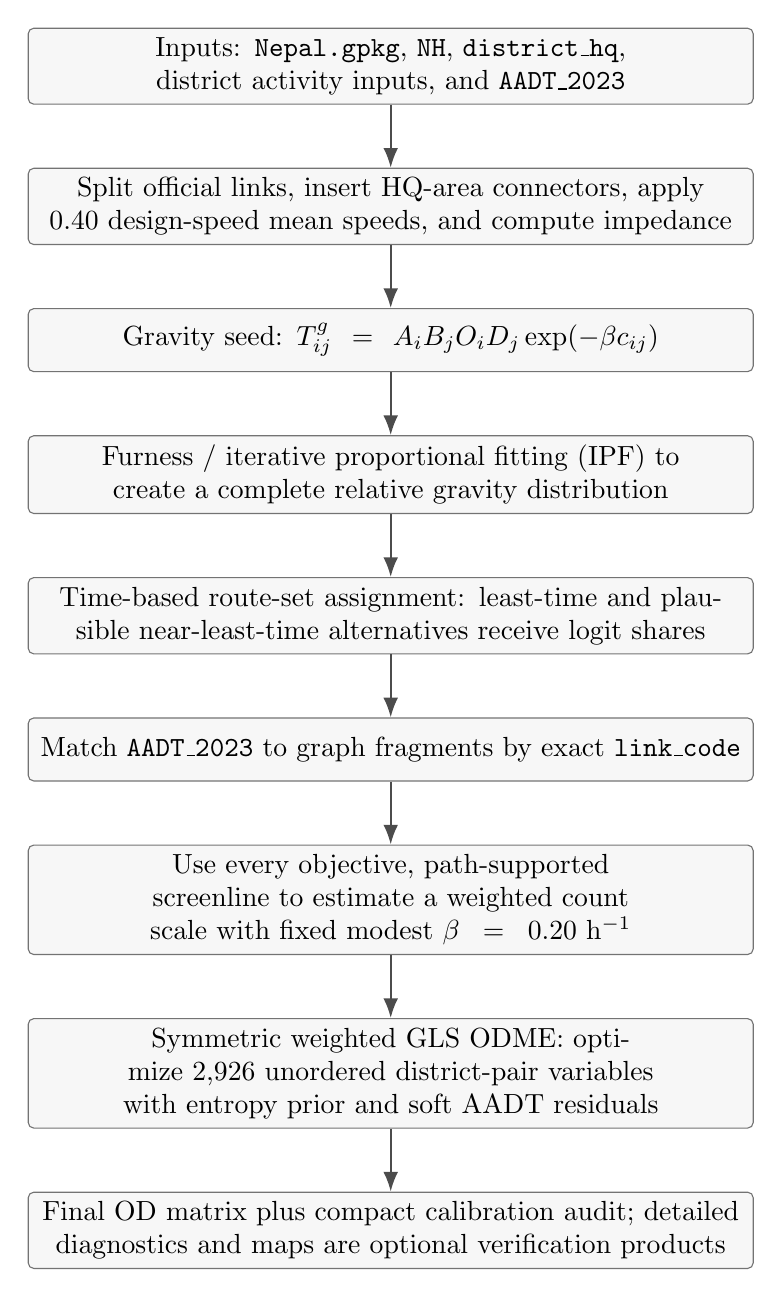
\begin{tikzpicture}[
  node distance=8mm,
  box/.style={rectangle, rounded corners=2pt, draw=black!55, fill=black!3,
              align=center, text width=0.74\linewidth, minimum height=8mm},
  arrow/.style={-{Latex[length=2.5mm]}, thick, draw=black!70}
]
\node[box] (input) {Inputs: \texttt{Nepal.gpkg}, \texttt{NH}, \texttt{district\_hq}, district activity inputs, and \texttt{AADT\_2023}};
\node[box, below=of input] (graph) {Split official links, insert HQ-area connectors, apply 0.40 design-speed mean speeds, and compute impedance};
\node[box, below=of graph] (seed) {Gravity seed: $T^{g}_{ij}=A_iB_jO_iD_j\exp(-\beta c_{ij})$};
\node[box, below=of seed] (ipf) {Furness / iterative proportional fitting (IPF) to create a complete relative gravity distribution};
\node[box, below=of ipf] (paths) {Time-based route-set assignment: least-time and plausible near-least-time alternatives receive logit shares};
\node[box, below=of paths] (targets) {Match \texttt{AADT\_2023} to graph fragments by exact \texttt{link\_code}};
\node[box, below=of targets] (scale) {Use every objective, path-supported screenline to estimate a weighted count scale with fixed modest $\beta=0.20$ h$^{-1}$};
\node[box, below=of scale] (odme) {Symmetric weighted GLS ODME: optimize 2,926 unordered district-pair variables with entropy prior and soft AADT residuals};
\node[box, below=of odme] (outputs) {Final OD matrix plus compact calibration audit; detailed diagnostics and maps are optional verification products};
\draw[arrow] (input) -- (graph);
\draw[arrow] (graph) -- (seed);
\draw[arrow] (seed) -- (ipf);
\draw[arrow] (ipf) -- (paths);
\draw[arrow] (paths) -- (targets);
\draw[arrow] (targets) -- (scale);
\draw[arrow] (scale) -- (odme);
\draw[arrow] (odme) -- (outputs);
\end{tikzpicture}
}
\caption{Implemented OD synthesis and calibration workflow.}
\label{fig:flow}
\end{figure}

\section{Gravity Seed Matrix}

Let $O_i$ be productions from origin zone $i$, $D_j$ be attractions to
destination zone $j$, and $c_{ij}$ be the inter-zonal impedance. The seed matrix
is generated by a doubly constrained gravity model, a standard trip-distribution
form in spatial interaction and transport modelling \cite{wilson1967,ortuzar2011}:

\begin{equation}
T^{g}_{ij}=A_iB_jO_iD_jf(c_{ij}), \qquad i\neq j,
\label{eq:gravity}
\end{equation}

with

\begin{equation}
f(c_{ij})=\exp(-\beta c_{ij}).
\label{eq:friction}
\end{equation}

The present dataset does not include an observed directional trip-production
and trip-attraction survey. Therefore, the initial gravity seed uses the same
district economic-activity prior on both sides:

\begin{equation}
O_i = D_i = A_i^{\text{activity}} = P_i\,g_{p(i)} .
\end{equation}

Here $P_i$ is the district population and $g_{p(i)}$ is the GDP-per-capita
multiplier for the province containing district $i$. The activity proxy is
therefore a district GDP proxy, recorded in \texttt{Input.xlsx} as
\texttt{activity\_proxy}, \texttt{Oi\_trips} and \texttt{Di\_trips}. The code
uses the explicit formula $P_i g_{p(i)}$ and treats the two trip-end columns as
the same symmetric prior, not as observed directional productions and
attractions. Population is sourced from the 2021 National Population and
Housing Census \cite{nso2021}, while the provincial GDP-per-capita values are
sourced from the National Statistics Office provincial accounts dataset
\cite{nso_gdppc}. The activity vector defines the relative spatial pattern of
the seed only; it is not interpreted as an observed daily production or
attraction. The initial row and column sums therefore describe the relative
gravity pattern used to shape the gravity prior; they are not observed or
enforced district trip-end constraints.

This GDP proxy has an important spatial limitation. Because $g_{p(i)}$ is the
same value for every district inside a province, the formula cannot capture
within-province variation in economic activity. A provincial capital and a
remote hill district in the same province receive the identical per-capita
economic multiplier, so all within-province differentiation collapses to
population. This is a recognized limitation of population-based GDP
disaggregation: Wang and Sun's gridded GDP downscaling work uses population
together with nighttime lights because nighttime-light information helps
reduce both the limitations of lights alone and the assumption of even GDP per
capita within an administrative boundary \cite{wangsun2022}. The present
district activity proxy should therefore be read as a transparent coarse prior,
not as a fine-grained district GDP observation.

Because no observed trip-length distribution is available, $\beta$ is treated
as a transparent planning assumption rather than asserted as a behavioural
constant. The current run fixes a modest deterrence value,
$\beta=0.20~\mathrm{h}^{-1}$, to avoid the overly steep prior produced when the
previous held-out highway validation selected $\beta=0.80~\mathrm{h}^{-1}$.
Sensitivity tests can still compare a capped candidate set:

\begin{equation}
\mathcal{B}=\{0.02,0.05,0.10,0.20\}\;\mathrm{h}^{-1}.
\label{eq:beta-selection}
\end{equation}

This is a prior-shape assumption, not a claim that AADT is an observed OD
trip-length distribution. The fixed value, candidate set and run mode are
recorded in the workbook controls and calibration log. The purpose is to keep
the seed matrix broad enough for a national district-level planning OD while
remaining explicit about the absence of a supporting trip survey
\cite{ortuzar2011}.

The balancing factors $A_i$ and $B_j$ are solved iteratively so that the seed
matrix respects the production and attraction totals:

\begin{equation}
\sum_j T^{g}_{ij}=O_i, \qquad \sum_i T^{g}_{ij}=D_j.
\label{eq:constraints}
\end{equation}

The implementation uses Furness balancing, also known as iterative proportional
fitting (IPF). At each iteration, rows are scaled to match productions and
columns are scaled to match attractions:

\begin{align}
T_{ij} &\leftarrow T_{ij}\frac{O_i}{\sum_j T_{ij}}, \\
T_{ij} &\leftarrow T_{ij}\frac{D_j}{\sum_i T_{ij}}.
\end{align}

This procedure is consistent with the classical Furness method
\cite{furness1965} and with entropy-based trip distribution formulations
\cite{wilson1967,morphet1975,ortuzar2011}. The diagonal cells are set to zero
because this matrix represents inter-district traffic assignment rather than
intra-zonal movements.

\section{Assignment Representation}

For each non-zero seed OD pair, the script first identifies the least-time path
using Dijkstra's algorithm and then retains up to three plausible time-based
alternatives. An alternative more than 25\% slower than the least-time path is
excluded. The retained paths receive fixed logit route shares based on their
travel-time difference \cite{ortuzar2011}. This produces a fractional
assignment-incidence matrix $P$:

\begin{equation}
p_{ar}=\sum_{k\in K_r}s_{rk}\,I(a\in k),
\qquad
s_{rk}=
\frac{\exp[-\theta(c_{rk}-c_{r\min})]}
{\sum_{h\in K_r}\exp[-\theta(c_{rh}-c_{r\min})]}.
\label{eq:incidence}
\end{equation}

Here $r$ indexes an OD pair, $a$ indexes an AADT calibration target, $K_r$ is
the retained route set, $c_{rk}$ is route travel time, $c_{r\min}$ is the
least route travel time, $s_{rk}$ is the route share, and $I(\cdot)$ equals one
when a route uses target $a$. The default route-choice sensitivity is
$\theta=2.0~\mathrm{h}^{-1}$. A workbook switch can use a single least-time
path for sensitivity testing. The modelled count at target $a$ is

\begin{equation}
\hat{y}_a = \sum_r p_{ar}x_r = (Px)_a,
\label{eq:count_equation}
\end{equation}

where $x_r$ is the OD demand for pair $r$. This is the core bridge between the
matrix and the AADT observations. It also makes clear that an AADT count is a
sum of many OD movements on a section, rather than a required value for one OD
cell.

\section{AADT Target Construction}

The first concern in this step was to avoid a misleading calibration. AADT
coverage is incomplete, and the count table does not provide direction. Missing
counts are therefore not interpreted as zero-flow observations. In addition,
not every observed AADT section is equally appropriate for district-level OD
matrix estimation. A highway section inside a district can carry local,
intra-district and urban traffic that the inter-district district-HQ matrix is
not designed to represent. The current calibration therefore uses
district-boundary screenline selection.

The current run uses the master \texttt{Nepal.gpkg} \texttt{NH} layer and the
\texttt{district\_boundary} layer directly. A road link is considered for the
soft screenline objective when it has a positive observed count and lies within
the configured district-boundary screenline buffer:

\begin{equation}
d_i \leq 500\text{ m}.
\end{equation}

Here $d_i$ is the projected distance from road link $i$ to the
\texttt{district\_boundary} linework, and $h_i$ is the projected distance from
road link $i$ to the nearest \texttt{district\_hq} area. The 500 m boundary
buffer allows for small geometric offsets between official highway geometry and
administrative boundary linework. Within this screenline set, primary targets
are links with \texttt{AADT\_2023} at least 1000 vehicles/day and $h_i\geq3000$
m. HQ-adjacent screenlines and lower-volume screenlines are retained as soft
evidence with larger GLS variance factors instead of being forced into a binary
keep/drop rule. Links outside the screenline buffer remain in the audit as
interior/local context AADT with default calibration weight zero. Every
path-supported screenline target with positive weight enters the ODME count
term. A link with no such path is retained in the audit with the explicit status
\texttt{no\_hq\_od\_path}; it is not removed because the seed happens to fit
or fail to fit it.

The model uses \texttt{AADT\_2023} as the two-way vehicle/day count target.
The field and target-selection controls are code defaults that can be configured
by adding or editing rows in \texttt{05\_OD\_Params}:
\texttt{aadt\_value\_field}, \texttt{aadt\_units},
\texttt{aadt\_source\_period}, \texttt{master\_gpkg}, \texttt{road\_layer},
\texttt{district\_hq\_layer}, \texttt{district\_boundary\_layer},
\texttt{screenline\_buffer\_m}, \texttt{screenline\_min\_hq\_distance\_m},
\texttt{min\_calibration\_aadt}, \texttt{screenline\_target\_weight},
\texttt{context\_target\_weight}, \texttt{gls\_category\_variance\_primary},
\texttt{gls\_category\_variance\_hq\_adjacent},
\texttt{gls\_category\_variance\_low\_volume},
\texttt{district\_prior\_log\_std}, \texttt{beta\_selection\_mode}, and
\texttt{beta\_candidates}. The candidate default weights are

\begin{equation}
w_i=
\begin{cases}
1, & \text{for primary, HQ-adjacent and low-volume screenline targets},\\
0, & \text{for interior/local context AADT links}.
\end{cases}
\end{equation}

Because \texttt{link\_code} is preserved from each official highway feature
onto every derived graph fragment, exact link-code matching is used. For a
selected \texttt{AADT\_2023} source link $a$, its selector is the set $E_a$ of
all graph fragments with the same unique code.
Incidence is

\begin{equation}
p_{ar}=1 \quad \text{if} \quad E_a\cap E_r\neq\emptyset ,
\end{equation}

where $E_r$ is the edge set of OD path $r$. Both graph directions are included,
so the resulting target is a two-way section count.

Each official \texttt{link\_code} is treated as its own calibration target. The
model does not combine adjacent active official sections into a corridor-level
maximum, sum, or average. Thus, if the Butwal--Gorusinghe corridor contains
\texttt{NH01-046}, \texttt{NH01-047}, \texttt{NH01-048}, \texttt{NH01-049}, and
\texttt{NH01-050}, each section contributes its own target only when it passes
the district-screenline rule. An OD path that crosses several active sections
contributes to each corresponding target selector separately.

After the count-scaled seed is assigned, the calibration applies an additional
ratio diagnostic before weighted GLS fitting. For a candidate target $a$, let
$\hat{y}^0_a$ be the modelled flow from the count-scaled seed and $y_a$ be the
observed AADT. If $\hat{y}^0_a$ is effectively zero while $y_a$ is large, the
station is flagged as a likely intra-city or local station rather than an
inter-district screenline. In the weighted GLS formulation this diagnostic
inflates the count variance instead of forcing a binary keep/drop decision:

\begin{equation}
\hat{y}^0_a \leq 1
\quad\text{or}\quad
\frac{\hat{y}^0_a}{y_a} \leq 0.01 .
\end{equation}

This is a diagnostic downweighting step, not a numerical clamp. The target
remains visible in \texttt{aadt\_target\_fit.csv}; when it is path-supported and
part of the soft screenline set, its seed-implausibility factor increases
$\sigma_a^2$ so that the count can pull the solution gently without dominating
the weighted GLS objective. Targets with no routed HQ-to-HQ path remain
unusable as constraints and are reported separately as \texttt{no\_hq\_od\_path}.

\begin{table}[H]
\centering
\caption{\texttt{AADT\_2023} target construction for the current OD calibration.}
\begin{tabularx}{\linewidth}{p{0.34\linewidth} X}
\toprule
\textbf{Item} & \textbf{Current treatment} \\
\midrule
Source field & \texttt{Nepal.gpkg}, layer \texttt{NH}, field
\texttt{AADT\_2023}. \\
Soft target rule & Positive \texttt{AADT\_2023} within 500 m of
\texttt{district\_boundary}; primary screenlines have
\texttt{AADT\_2023} at least 1000 vehicles/day and are at least 3000 m from the
nearest \texttt{district\_hq} area. HQ-adjacent and lower-volume screenlines are
kept with inflated GLS variance. \\
ODME target count & Reported in the completed run audit after objective
screenline selection and routed-path support are checked. \\
Context rows & Interior/local links outside the district-boundary screenline
buffer remain in the audit with default weight zero. \\
Target identity & One calibration target per official \texttt{link\_code};
adjacent sections are not collapsed into a corridor maximum, sum or average. \\
Graph selector & All \texttt{GraphEdges} fragments whose copied
\texttt{code} field matches the source \texttt{link\_code}. \\
Path incidence & An OD pair contributes to target $a$ through the sum of its
alternative-route shares that use selector $E_a$. \\
Default audit & \texttt{calibration\_log.csv} and
\texttt{aadt\_target\_fit.csv}. \\
Optional diagnostics & Detailed path, mapping, station-fit, seed and pair
tables are written only when the corresponding workbook switches are enabled. \\
\bottomrule
\end{tabularx}
\end{table}

Because the AADT rows are non-directional, the current calibration treats them
as two-way section/screenline information. Directional calibration would require
directional AADT or explicit directed graph-edge IDs.

\subsection{Objective Screenline Handling}

The matrix has one zone at each district headquarters, so it represents
inter-district HQ-to-HQ movement rather than every local movement on the
national highway network. The geographic district-boundary rule identifies the
screenline set; minimum-count and HQ-distance checks classify those screenlines
into primary, low-volume and HQ-adjacent evidence classes with different GLS
variance factors. This classification depends only on the source geometry and
observed AADT, never on agreement between a road count and the gravity seed.

Every positive-weight screenline with at least one routed HQ-to-HQ OD path
enters the count term. A screenline with no routed path remains in
\texttt{aadt\_target\_fit.csv} with the status
\texttt{no\_hq\_od\_path}. It cannot constrain the HQ-to-HQ matrix, but it is
important evidence about the limits of the present zone and network
representation. Context AADT rows likewise remain visible with zero default
weight; they are not interpreted as observed zero demand.

\section{Direct District-Level OD Estimation}

Traffic counts constrain flows across roads, not individual district-to-district
trips. With 77 districts, the model contains 2,926 unordered inter-district
pair variables, mirrored into 5,852 off-diagonal matrix cells for CSV
compatibility. The available AADT evidence contains far fewer independent
screenline observations. The problem is consequently under-identified, but its
geography remains district-to-district throughout: the model estimates every
district pair directly and uses the gravity matrix as a transparent prior.
This is a regularized count-based OD estimation approach consistent with the
maximum-likelihood/entropy foundation of Van Zuylen and Willumsen
\cite{vanzuylen1980} and Spiess \cite{spiess1987}, but the current implemented
calibration is a weighted generalized least-squares extension rather than a hard
ME2 exact-count-matching formulation.

Let $x^g_q$ be the unscaled symmetric gravity seed for unordered district pair
$q=\{i,j\}$, where $i\ne j$. The seed is placed in daily vehicle units with the
weighted screenline scale

\begin{equation}
s=\frac{\sum_{r\in A^\ast}w_r g_r y_r/\sigma_r^2}
        {\sum_{r\in A^\ast}w_r g_r^2/\sigma_r^2},
\qquad x^0_q=s x^g_q,
\label{eq:district-target-scale}
\end{equation}

where $g_r$ is the flow assigned from the unscaled gravity seed to objective
screenline $r$, $y_r$ is its two-way AADT, and $w_r$ is its calibration weight.
The count uncertainty is

\begin{equation}
\sigma_r=\max\left(\sqrt{y_r},\;0.20y_r\right).
\label{eq:district-count-variance}
\end{equation}

For each unordered district pair, the mirrored matrix values are

\begin{equation}
x_{ij}=x_{ji}=x_q,\qquad i\ne j.
\label{eq:symmetric-demand}
\end{equation}

Let $P_{rq}$ denote the two-way assignment incidence from unordered pair $q$ to
screenline $r$. It is obtained by summing the route incidences of the two
mirrored directions, using the time-based route alternatives described above,
and is fixed during a calibration run. The modelled count is

\begin{equation}
\hat{y}_r = \sum_q P_{rq}x_q.
\label{eq:district-odme}
\end{equation}

Before beta selection, count scaling, seed-implausibility diagnostics and GLS
calibration, AADT targets are screened for path-incidence duplication. This is
not a geographic proximity rule. For each pair of candidate stations $a$ and
$b$, the implementation compares their OD-pair incidence vectors
$P_{a\cdot}$ and $P_{b\cdot}$. Let
$S_a=\{q:P_{aq}>\epsilon\}$. Two stations are connected into the same corridor
group when both

\begin{equation}
J(a,b)=\frac{|S_a\cap S_b|}{|S_a\cup S_b|}\ge 0.98
\end{equation}

and

\begin{equation}
C(a,b)=
\frac{P_{a\cdot}P_{b\cdot}}
{\|P_{a\cdot}\|\|P_{b\cdot}\|}
\ge 0.98 .
\end{equation}

Connected components under this incidence-similarity rule become corridor
groups. A group $G$ is then represented by one super-constraint:

\begin{equation}
y_G=\operatorname{median}_{a\in G}(y_a),\qquad
P_{Gq}=\max_{a\in G}P_{aq}.
\end{equation}

Thus a route crossing several nearly identical stations contributes to one
shared corridor residual rather than several duplicate count residuals. This
prevents stacking adjacent measurements of the same path-incidence screenline,
while retaining independent stations whose OD-pair incidence vectors diverge.
The seed-implausibility ratio diagnostic is then run after this grouping step
on the collapsed constraint set.

Calibration is then performed as a weighted generalized least-squares ODME
problem with an entropy prior around the count-scaled gravity matrix. This is
not a hard ME2 formulation: the entropy term keeps the solution close to the
gravity prior, but the AADT observations enter as weighted residuals rather than
as equality constraints. This follows the GLS OD-matrix estimation tradition of
Cascetta \cite{cascetta1984} and the practical gradient/count-adjustment
approach of Spiess \cite{spiess1990}:

\begin{equation}
Z(x)=
\sum_q x_q\left[\ln\left(\frac{x_q}{x_q^0}\right)-1\right]+x_q^0
+\frac{1}{2}\sum_r w_r\left(\hat{y}_r-y_r\right)^2,
\qquad
\hat{y}_r=\sum_q P_{rq}x_q .
\label{eq:weighted-gls-odme}
\end{equation}

The count weight is $w_r=1/\sigma_r^2$. The implemented variance inflates the
basic count uncertainty using path dilution, target category and
seed-implausibility terms:

\begin{equation}
\sigma_r^2 =
\sigma_{\text{count},r}^2
\left(\frac{n_{\text{pairs},r}}{\bar{n}}\right)_+
c_r
s_r ,
\end{equation}

where $\sigma_{\text{count},r}=\max(\sqrt{y_r},0.20\max(y_r,1000))$,
$n_{\text{pairs},r}$ is the number of OD-pair variables crossing the target,
$c_r$ is a target-category variance factor, and
$s_r=\max(1,|\ln(y_r/\hat{y}_r^0)|)$ is the seed-implausibility factor.
Clearly interior/local AADT rows remain excluded. Primary, HQ-adjacent and
low-volume district screenlines are retained as soft evidence, so an ambiguous
or locally contaminated count can pull the matrix without forcing exact
equality.

The route-incidence rank is retained in the calibration log as a structural
diagnostic. It is expected to be much lower than 2,926 because road counts
observe overlapping combinations of OD pairs; this is exactly why the
count-scaled gravity prior is necessary.

\subsection{Calibration Scope}

The gravity deterrence coefficient is fixed at the modest value
$\beta=0.20~\mathrm{h}^{-1}$ before district estimation. AADT supplies aggregate
road-use evidence, while population and economic activity supply only the
relative pattern used for the gravity prior; neither is a direct district OD
survey.

The final values are best described as:

\begin{quote}
Estimated daily inter-district vehicles obtained by calibrating symmetric
district-pair variables to selected two-way \texttt{AADT\_2023} screenlines,
with a count-scaled gravity matrix used as the prior.
\end{quote}

For reporting and MLPI transfer, \texttt{od\_matrix.csv} is written directly to
two decimal places. Mirrored cells should be read as the same symmetric
district-pair estimate, not as independently observed directional flows. An
individual OD cell is not expected to equal a road section's AADT, because the
latter aggregates all assigned OD movements using that section.

\section{Calibration Diagnostics}

\begin{table}[H]
\centering
\caption{Direct district-level ODME configuration and audit fields.}
\begin{tabularx}{\linewidth}{L{0.43\linewidth} Y}
\toprule
\textbf{Diagnostic} & \textbf{Value} \\
\midrule
Symmetric district-pair variables & 2,926 (77 $\times$ 76 / 2) \\
Mirrored off-diagonal matrix cells & 5,852 (77 $\times$ 76) \\
Calibration formulation & Weighted GLS ODME with entropy prior and soft AADT
residuals; not hard ME2 exact-equality count matching
\cite{cascetta1984,spiess1990}. \\
District-screenline AADT candidates & 445 graph-matched target rows, collapsed
by path-incidence similarity to 304 screenline/corridor constraints. \\
Path-supported objective targets & 214 soft GLS objective targets; 90
screenline constraints have no routed HQ-to-HQ path. \\
Seed-implausibility downweighted targets & 12 targets receive inflated GLS
variance from the seed-ratio diagnostic; zero targets are hard-excluded by this
diagnostic. \\
Selected beta and validation RMSE / WAPE & Fixed modest $\beta=0.20~\mathrm{h}^{-1}$;
validation RMSE 4,439.61 and WAPE 0.6469. \\
AADT coefficient-of-variation floor & 0.20 \\
GLS variance factors & Primary screenline 1.0; HQ-adjacent 16.0; low-volume
and context 100.0; path-dilution power 1.0; seed-implausibility floor 1.0;
resulting $\sigma$ range 200.40--38,636.66 vehicles/day. \\
Route-choice representation & Up to three logit-shared time paths \\
District incidence rank & 208 \\
Initial / final count RMSE, GEH and OD total & RMSE 4,332.14 $\rightarrow$
4,332.79; mean GEH 33.34 $\rightarrow$ 33.22; OD total 42,461.53 $\rightarrow$
42,472.37 vehicles/day. \\
Weighted GLS solver status, reason and iterations & \texttt{weighted\_gls\_converged};
\texttt{weighted\_gls\_lbfgsb}; convergence by relative objective reduction;
165 iterations. \\
\bottomrule
\end{tabularx}
\end{table}

The completed direct run writes its values to \texttt{calibration\_log.csv},
\texttt{aadt\_target\_fit.csv} and \texttt{od\_matrix.csv}. The log records
the weighted prior scale, beta-selection audit, district-incidence rank, GLS
iterations, variance controls, seed-implausibility diagnostics, the selected final
row, and the final \texttt{fit\_status} and \texttt{stop\_reason}. The fit
audit reports raw RMSE for count-scale context, standardized residuals, GEH as
a familiar traffic-assignment diagnostic, and
\texttt{seed\_to\_observed\_ratio} for identifying city/local count
constraints. These measures are calculated for the path-supported objective
screenlines. The audit also lists objective screenlines with no routed
HQ-to-HQ path and targets whose seed-implausibility factor was inflated, so
they are not mistaken for failed ODME constraints.

A status of \texttt{weighted\_gls\_converged} means that the weighted
entropy-plus-count objective reached the numerical optimizer criterion. It does
not mean every observed count is reproduced closely; low-trust or highly shared
counts are intentionally fitted softly. Count fit, GEH, residual patterns, GLS
weights and the largest district-pair movements should be reviewed together
before the matrix is used for MLPI. The estimate remains a transparent,
count-informed planning matrix, rather than a replacement for a surveyed OD
matrix.

\section{Map-Based Verification}

Two verification maps were generated to make the calibration auditable:

\begin{enumerate}
    \item an AADT map showing \texttt{AADT\_2023} sections from
    \texttt{Nepal.gpkg}, labelled by link code and AADT; and
    \item a major-OD map showing the largest final symmetric OD cells along their
    least-time representative road paths.
\end{enumerate}

Only the two PDF figures referenced below are required for reporting. SVG, PNG
and interactive HTML map variants are not part of the current output set.
The reproducible verification workflow is implemented in
\texttt{/Project/code/od\_verification.py}; its report-ready PDF outputs are
written directly to \texttt{/Project/output/OD}.

Each figure contains a national overview and separate western, central, and
eastern panels. Detailed panels use small collision-filtered labels. The map
geometry is simplified only for display; matching, assignment, calibration,
and reported values use the original network geometry.

The routed OD map does not use straight desire lines or a separate illustrative
road layer. For each displayed OD cell, the verification workflow recomputes
the least-time representative path on \texttt{GraphEdges.gpkg} using
\texttt{travel\_time\_hours}, the same edge weight used by the OD calibration.
The calibration itself distributes demand over a small alternative route set;
the map shows the least-time member of that set so the figure remains legible.
The graph was derived from \texttt{Nepal.gpkg} and is the same network
representation used to calculate the impedance matrix. The displayed line is
therefore an estimated routed OD movement, rather than an independently
observed ``actual'' OD trip.

\begin{figure}[H]
\centering
\figurepanel{figures/aadt_nh_pcu_overview_regions.pdf}{AADT\_2023 on Nepal.gpkg highway sections.}
\caption{Two-way AADT from \texttt{Nepal.gpkg}, layer \texttt{NH}, field
\texttt{AADT\_2023}, expressed in vehicles/day.
This figure is produced by the verification-map workflow.}
\label{fig:aadtmap}
\end{figure}

\begin{figure}[H]
\centering
\figurepanel{figures/major_od_routed_paths_overview_regions.pdf}{Top final OD movements on modelled shortest paths.}
\caption{Largest symmetric OD matrix cells plotted along their modelled
shortest paths. A label is an OD-matrix value, not an aggregate
link volume. Shared road sections may therefore carry several labelled OD
movements.}
\label{fig:odmap}
\end{figure}

\section{Outputs}

\begin{table}[H]
\centering
\caption{Default output files from the current OD run.}
\begin{tabularx}{\linewidth}{p{0.36\linewidth} X}
\toprule
\textbf{Output} & \textbf{Meaning} \\
\midrule
\texttt{gravity\_seed\_matrix.csv} &
Pre-calibration symmetric gravity seed written before AADT count-scaling and
ODME. It is useful for inspecting the activity-and-impedance pattern of the
seed, and should not be read as calibrated daily traffic. Values are reported
to two decimal places. \\
\texttt{od\_matrix.csv} &
Final OD matrix used by MLPI. Rows and columns are ordered alphabetically and
labelled as \texttt{District | HQ}, without a serial-number prefix. Values are
reported as expected daily demand to two decimal places. Mirrored cells carry
the same symmetric district-pair value. \\
\texttt{calibration\_log.csv} &
Compact count-term, beta-selection, district-incidence, weighted-GLS solver,
seed-implausibility and selected-final audit. \\
\texttt{screenline\_grouping\_report.csv} &
Incidence-similarity grouping audit. Each original AADT target is listed with
its assigned corridor group, member link codes, representative group AADT, and
minimum within-group Jaccard/cosine overlap. \\
\texttt{aadt\_target\_fit.csv} &
Final fit audit for every collapsed district-screenline
\texttt{AADT\_2023} constraint, including path-support status, zero-seed
diagnostic/downweighting note, final assigned flow, GLS sigma and GLS weight
for selected calibration targets. \\
\texttt{seed\_od\_matrix.csv} &
Beta-selected, count-scaled gravity-prior matrix used directly by ODME, with
the same alphabetic district/HQ label format and two-decimal values. \\
\texttt{optional diagnostics} &
The ID-labelled matrix, ID-labelled seed matrix, OD-pair tables,
path-incidence features, mapping reports, station-fit reports and summary text
are written only when
workbook switches such as \texttt{write\_id\_matrix},
\texttt{write\_diagnostics}, \texttt{write\_seed\_outputs},
\texttt{write\_pair\_table}, and \texttt{write\_summary} are enabled. \\
\bottomrule
\end{tabularx}
\end{table}

\section{Interpretation and Limitations}

The current matrix combines network impedance, a relative district activity
pattern and observed traffic counts. The strongest part of the method is that
AADT observations are retained as observations only where they exist.
Unobserved links remain unconstrained.

The main limitations are:

\begin{itemize}
    \item Link-count calibration is underdetermined: several district OD
    matrices can reproduce similar AADT values. The 2,926 unordered
    district-pair variables are estimated directly, but the count-scaled
    gravity matrix remains necessary as a prior. The result is a
    prior-constrained estimate, not an observed OD survey.
    \item The \texttt{AADT\_2023} field is non-directional, so calibration
    remains two-way section/screenline calibration even though link-code
    matching is exact. The final OD matrix is symmetric and should not be
    described as directional.
    \item District-boundary and HQ-distance filtering reduce local/intra-district
    AADT contamination, but they cannot fully separate through inter-district
    traffic from all local traffic near administrative boundaries. The
    seed-implausibility diagnostic flags candidate stations whose count-scaled
    seed flow is effectively zero while observed AADT is large; those retained
    as soft constraints receive inflated GLS variance rather than being hidden
    by numerical clamping.
    \item Assignment distributes an OD pair over a small fixed set of
    time-based alternatives. It does not include congestion feedback or a
    dynamic equilibrium route-choice model.
    \item The gravity seed uses the same district GDP proxy for its origin and
    destination weights because directional trip-end observations are not
    available. It defines the relative prior pattern, not observed district
    trip-end totals.
    \item The GDP proxy uses provincial GDP per capita for every district in a
    province. It cannot capture within-province economic concentration beyond
    the population term, so a provincial capital and a remote district in the
    same province receive the same per-capita multiplier.
    \item The gravity seed is dense, so it creates very small expected values
    between many distant or weakly related district pairs. These low cells are
    treated as modelled expectations, not as observed individual trips.
    \item The compact audit reports active calibration targets. Detailed
    unmatched-target and path-incidence checks should be enabled when preparing
    verification maps or investigating a network rebuild.
    \item The impedance uses 40\% of source design speed as average operating
    speed. It still does not explicitly represent congestion, pavement
    condition, weather or seasonal closure.
    \item District-HQ connectors now use the \texttt{Nepal.gpkg}
    \texttt{district\_hq} area geometry directly. A large connector distance is
    a network-access QA item, not evidence that the HQ was a disconnected point.
    \item The activity proxy is not a direct observation of district trip ends.
    District travel surveys, origin--destination interviews, mobile-device
    movement data, freight surveys, directional cordon counts, and additional
    AADT screenlines would add independent district-level constraints and allow
    a more locally responsive calibration.
    \item The selected gravity deterrence parameter is validated against held-out
    highway-family counts, not against observed OD trip-length data. It remains
    a count-informed prior parameter rather than a behavioural survey estimate.
\end{itemize}

The most valuable future data additions are directional and multi-day AADT
counts, observed operating speeds, district trip-end observations, and
explicit local-road access connectors beyond the national-highway graph. Each
would improve a different part of the estimate: counts strengthen calibration,
trip-end data strengthen the district prior and constraints, operating speeds
strengthen route impedance, and local-road data strengthen route alternatives.

\section{Conclusion}

The final OD matrix should be described as a calibrated daily inter-district
HQ-to-HQ demand matrix in the same units as the objective, path-supported AADT
evidence. With the current
configuration, that evidence is \texttt{AADT\_2023} from
\texttt{Nepal.gpkg}. Methodologically, the estimate is not just a gravity
matrix and it is not a forced copy of AADT values. It calibrates symmetric
district-pair variables to AADT with a weighted GLS objective and a
count-scaled gravity prior.
The revised implementation keeps the impedance graph tied to \texttt{Nepal.gpkg}, uses
the \texttt{district\_hq} area layer for closest-point HQ connectors, applies
the \texttt{NH} design-speed field with a 0.40 mean-speed factor for
travel-time impedance, and constructs AADT selectors from exact
\texttt{Nepal.gpkg} \texttt{NH} link codes.

\part{MLPI Junction-Link Prioritization}

\section{Purpose and Position in the Workflow}

The MLPI workflow begins after the impedance and OD stages. It does not create
a synthetic OD matrix. Instead, \texttt{mlpi.py} reads the calibrated ODME output
\texttt{/Users/bishalbhurtel/Desktop/Project/output/OD/od\_matrix.csv} and
uses it as the demand surface for road-link consequence scoring.

The purpose of the MLPI calculation is to rank national-highway road links by
the consequence of losing that link. A scored link is not an arbitrary short
geometry fragment. The script first builds an analytical graph from
\texttt{Nepal.gpkg}, layer \texttt{NH}, then aggregates the graph into
non-overlapping junction-to-junction road links. Each of those links is tested
one at a time. The resulting score is a consequence-based priority index:

\begin{equation}
\mathrm{MLPI}_{\ell}
=w_P P_{\ell}+w_S S_{\ell}+w_E E_{\ell}+w_I I_{\ell},
\label{eq:mlpi-final}
\end{equation}

where $\ell$ is a scored road link, $P$ is the physical dimension, $S$ is the
social dimension, $E$ is the economic dimension, and $I$ is the
interconnectedness / airport-access dimension. The current workbook selects
the tentative top-level weights

\begin{equation}
(w_P,w_S,w_E,w_I)=(0.35,0.25,0.25,0.15),
\end{equation}

and the code normalizes top-level weights if a different workbook scheme is
selected. The workbook also contains an AHP weight set, but the current
\texttt{01\_Run\_Config} selector is \texttt{Tentative}.

The model should be read as a comparative prioritization tool. A high MLPI
value means that, relative to the other tested road links in the same run, that
link produces larger travel-time, population-access, economic-access or
airport-access consequences when it is unavailable. It is not an observed
failure probability and it is not a direct monetary-loss estimate.

\section{Inputs Read by \texttt{mlpi.py}}

\texttt{mlpi.py} reads a small set of current project inputs:

\begin{table}[H]
\centering
\caption{Main MLPI inputs and how they are used.}
\small
\begin{tabularx}{\linewidth}{L{0.30\linewidth} Y}
\toprule
\textbf{Input} & \textbf{Use in MLPI} \\
\midrule
\texttt{Input.xlsx}, \texttt{01\_Run\_Config} &
Output folder, map switches, random seed, weight-scheme selector, master
GeoPackage path and ODME matrix path. \\
\texttt{Input.xlsx}, \texttt{02\_Network\_Params} &
Road-layer filter, AADT field, mean-speed factor, free-flow assignment controls
and disconnected-OD penalty. \\
\texttt{Input.xlsx}, \texttt{03\_Weights} &
Top-level MLPI weights and the active sub-dimension weights. \\
\texttt{Input.xlsx}, \texttt{04\_Model\_Params} &
Border-access decay, detour credit, regional balancing, air-access parameters
and related scenario constants. \\
\texttt{Input.xlsx}, \texttt{06\_Border\_Trade} &
Border-gateway coordinates and trade-volume weights for economic-access loss. \\
\texttt{Input.xlsx}, \texttt{07\_Population\_GDP} &
District population, GDP-per-capita and district anchor coordinates used for
population/GDP allocation and OD-zone mapping. \\
\texttt{Nepal.gpkg}, layer \texttt{NH} &
Authoritative highway geometry, design speeds and \texttt{AADT\_2023}. \\
\texttt{Nepal.gpkg}, layers \texttt{airport} and \texttt{air\_routes} &
Operational-airport points and observed domestic air-route links used to
represent limited air fallback when road-only travel is broken by a failed
link. \\
\texttt{Nepal.gpkg}, layers \texttt{district\_hq},
\texttt{national\_boundary} and \texttt{district\_boundary} &
District-headquarter anchors, labels and boundary context. \\
\texttt{od\_matrix.csv} &
External calibrated symmetric ODME matrix. Its row/column labels are parsed as
\texttt{District | HQ}. \\
\texttt{Airport Table.rtfd} &
Optional local airport registry used for display codes and operational status.
The airport geometries themselves still come from \texttt{Nepal.gpkg}. \\
\bottomrule
\end{tabularx}
\normalsize
\end{table}

The active traffic field is \texttt{AADT\_2023}, expressed in vehicles/day.
The current road filter is
\texttt{ALL}, so the full \texttt{NH} layer supplied in \texttt{Nepal.gpkg} is
available to the MLPI graph.

For MLPI, direction is not used as an independent scoring dimension. Link
criticality is driven by the total OD demand affected by a failed link and the
resulting travel-time or access consequence. A symmetric ODME matrix is
therefore sufficient for the current Hansen--Koks-style economic/access
scoring, provided it is reported honestly as symmetric daily demand rather than
as observed directional flow.

\section{Graph Construction}

\subsection{Road-edge preparation}

The road graph begins with \texttt{Nepal.gpkg}, layer \texttt{NH}. The script
requires usable \texttt{link\_len}, design-speed and AADT fields. The official
\texttt{link\_len} attribute is treated as the source length for each highway
feature:

\begin{equation}
L_f^{\mathrm{attr}}=\texttt{link\_len}_f .
\label{eq:mlpi-edge-length}
\end{equation}

When an official feature is split at junctions, the feature's official length
is allocated to the split segment in proportion to its share of the feature
geometry:

\begin{equation}
L_e=L_f^{\mathrm{attr}}
\frac{G_e}{\sum_{m\in f}G_m},
\label{eq:mlpi-segment-length}
\end{equation}

where $G_e$ is the geometric length share of split segment $e$ inside source
feature $f$. In other words, the coordinate geometry is used to divide the
official source length after noding; it is not used as the primary road-length
authority.

Each road edge receives the same average operating speed already documented in
Equation~\ref{eq:mean-speed}:

\begin{equation}
V_{\mathrm{avg},e} = 0.40 V_{d,e}.
\label{eq:mlpi-speed}
\end{equation}

The road-edge free-flow time is then

\begin{equation}
t_e=\frac{L_e}{V_{\mathrm{avg},e}}.
\label{eq:mlpi-road-time}
\end{equation}

This avoids introducing a second speed assumption inside MLPI. The speed term is
the same $V_{\mathrm{avg}}$ used by the impedance model. The current BPR
congestion parameter is \texttt{BPR\_ALPHA = 0}, so the active physical scoring
is a free-flow shortest-path consequence calculation.

AADT is read from \texttt{AADT\_2023}. If a valid positive value is present, it
is stored on the graph edge with a provenance label such as
\texttt{Nepal.gpkg NH AADT\_2023}. The current input is expected to carry this
required field.

\subsection{Topology and airport access}

The source road features are split at shared rounded coordinates so that true
junctions become graph nodes. Node coordinates are rounded to the configured
\texttt{endpoint\_precision} before shared endpoints are detected. No extra
topology-gap connectors are inserted by the current MLPI script; the repaired
\texttt{Nepal.gpkg} topology is treated as the road-network topology.

Airport points from the \texttt{airport} layer are connected to the nearest
road node so that a road traveller can reach an operational airport. The
\texttt{air\_routes} layer then supplies observed domestic air links between
airport pairs. These links are not treated as normal highway capacity. They are
reserved for the physical-dimension failure test as a last-resort alternative
when a road failure breaks the road-only path between an OD pair.

For an air-route edge between airports $a$ and $b$, the generalized air cost is

\begin{equation}
t^{\mathrm{air}}_{ab}
=\tau_{\mathrm{air}}+\kappa_{\mathrm{air}}
\frac{L_{ab}}{V_{\mathrm{air}}},
\label{eq:mlpi-air-cost}
\end{equation}

with current workbook parameters $V_{\mathrm{air}}=400$ km/h,
$\kappa_{\mathrm{air}}=10$, and $\tau_{\mathrm{air}}=4$ h. The value
$V_{\mathrm{air}}=400$ km/h is a conservative ATR 72 block-speed approximation:
ATR's technical sheet reports a 510 km/h maximum cruise speed and 300 NM block
time of 84 min, which is approximately 397 km/h over the block distance
\cite{atr2020}. The multiplier and fixed penalty are not calibrated Nepal
coefficients. They encode the air-mode penalty recommended by airport-choice
and generalized-cost literature, where access time, access cost, flight time,
waiting, reliability, check-in, security and gate processes are separate
disutility components \cite{kouwenhoven2008,koster2011,adler2005,acrp2015}.
The large multiplier deliberately keeps air travel from erasing road-failure
consequences too easily.

\section{Scored Failure Units}

The current run uses \texttt{build\_junction\_links()} to define the ranked
units. The road graph is simplified into continuous paths between nodes whose
degree is not two. These endpoints are ordinary road junctions, branch points
or dead ends. A pure ring would have no natural endpoint, so the code inserts
one deterministic break so that every physical road edge is assigned exactly
once.

For a scored link $\ell$, let $E_{\ell}$ be the set of physical road edges in
that continuous path. Its length and mean AADT are

\begin{align}
L_{\ell} &= \sum_{e\in E_{\ell}} L_e, \\
\bar{A}_{\ell}
&=\frac{\sum_{e\in E_{\ell}} A_e L_e}
        {\sum_{e\in E_{\ell}} L_e}.
\label{eq:mlpi-link-aadt}
\end{align}

The model-speed value reported for the link is also length-weighted:

\begin{equation}
\bar{V}_{\ell}
=\frac{\sum_{e\in E_{\ell}} V_{\mathrm{avg},e} L_e}
        {\sum_{e\in E_{\ell}} L_e}.
\label{eq:mlpi-link-speed}
\end{equation}

The link also receives an ID such as \texttt{LNK0001}, a display name based on
the dominant road reference and nearby place labels, a direct end-to-end
distance, a route-detour ratio $L_{\ell}/L^{\mathrm{direct}}_{\ell}$, a
dominant terrain zone, a dominant AADT source and other audit fields. The
junction-link list is written to
\texttt{output/MLPI/junction\_links\_used.csv}.

\section{Socioeconomic Allocation}

The social, economic and airport-access dimensions need population and GDP
weights on road nodes. \texttt{mlpi.py} conserves district totals from
\texttt{07\_Population\_GDP} by distributing each district's population and GDP
over representative road nodes. The current cap is 24 representative nodes per
district.

If the district polygon contains road nodes, the script selects a spread of
nodes inside that district. Settlement centroids can weight this split when a
settlement layer is present. In the current GeoPackage, that layer is not active,
so the ``otherwise'' branch below is the relevant current behaviour. For
district $z$ and selected road node $n$, the raw allocation weight is

\begin{equation}
r_{zn} =
\begin{cases}
0.25+s_{zn}, & \text{if settlement centroids are available},\\
1, & \text{otherwise},
\end{cases}
\label{eq:mlpi-allocation-raw}
\end{equation}

where $s_{zn}$ is the number of settlement centroids assigned to selected node
$n$. The share is

\begin{equation}
\alpha_{zn}=\frac{r_{zn}}{\sum_{m\in N_z} r_{zm}}.
\label{eq:mlpi-allocation-share}
\end{equation}

The allocated node population and GDP-weight are

\begin{align}
\mathrm{pop}_n &\leftarrow \mathrm{pop}_n+\alpha_{zn}\mathrm{Pop}_z,\\
\mathrm{gdp}_n &\leftarrow \mathrm{gdp}_n+
\alpha_{zn}\mathrm{Pop}_z\,\mathrm{GDPpc}_z .
\label{eq:mlpi-node-gdp}
\end{align}

If a district polygon cannot provide suitable road nodes, the district anchor
coordinate from the workbook is assigned to the nearest representative road
nodes. The script checks that total allocated population equals the total
district population. The allocation audit is written to
\texttt{output/MLPI/population\_node\_allocation.csv}.

\section{OD Matrix Loading and Zone Mapping}

The ODME matrix is read as a square CSV with matching row and column labels.
The script enforces these checks before scoring:

\begin{itemize}
    \item row and column labels must be unique;
    \item the row-label set must match the column-label set;
    \item all cells must be finite numeric values;
    \item negative demands are not allowed; and
    \item diagonal cells are set to zero.
\end{itemize}

Before physical path scoring, OD cells below the workbook control
\texttt{MIN\_OD\_PAIR\_DEMAND} are excluded. The current value is
1 vehicle/day. This threshold removes the very small dense-gravity tail from
MLPI routing while retaining the demand-bearing district pairs.

Labels are parsed in the current reporting form
\texttt{District | HQ}. Each zone is mapped to an MLPI road node using, in
order, the district's conserved socioeconomic allocation and then the
district/HQ anchor coordinate. The mapping is not hidden: it is written to
\texttt{output/MLPI/odme\_zone\_mapping.csv}.

Positive OD cells whose origin and destination map to the same road node are
skipped because they cannot load an inter-node road path. For the remaining
positive pairs, the demand is

\begin{equation}
q_{ij}=q_{ji}
= \text{symmetric ODME demand in vehicles/day for district pair }\{i,j\}.
\end{equation}

Only OD pairs connected on the baseline MLPI road graph contribute to physical
total-system-travel-time loss. Baseline-disconnected mapped pairs are retained
in the audit table \texttt{odme\_pairs\_used.csv} with a skip reason, because
they usually indicate a network-connectivity or zone-mapping issue that should
be reviewed separately.

\section{Normalization and Weighting}

Each raw sub-score is min-max normalized across the set of tested links:

\begin{equation}
\widetilde{x}_{\ell} =
\begin{cases}
\dfrac{x_{\ell}-\min_m x_m}{\max_m x_m-\min_m x_m},
& \max_m x_m > \min_m x_m,\\[8pt]
0, & \text{otherwise}.
\end{cases}
\label{eq:mlpi-minmax}
\end{equation}

This means the final MLPI ranking is relative to the links tested in the same
run. If every link has the same raw value for a sub-dimension, that normalized
sub-dimension contributes zero because it cannot distinguish priorities.

\section{Physical Dimension}

The physical score measures road-network travel-time consequence. It is the
dimension most directly tied to the calibrated ODME matrix and to the
free-flow link-removal idea used in link criticality studies
\cite{almotahari2019}.

The baseline physical graph is road-only:

\begin{equation}
R=(N,E_R), \qquad e\in E_R \text{ only if } e \text{ is a road edge}.
\end{equation}

That baseline choice is deliberate. The ODME matrix represents ordinary
inter-district movement on the highway network, so routine baseline trips are
not allowed to choose air routes simply because a direct flight looks faster.
For every connected OD pair $(i,j)$, Dijkstra's algorithm finds the baseline
minimum-time road path. The baseline OD travel time is

\begin{equation}
t^0_{ij}=\min_{p\in\mathcal{P}_{ij}}\sum_{e\in p} t_e,
\label{eq:mlpi-base-path}
\end{equation}

and baseline total system travel time is

\begin{equation}
\mathrm{TSTT}^0=\sum_{(i,j)\in\Omega^0} q_{ij}t^0_{ij},
\label{eq:mlpi-tstt-base}
\end{equation}

where $\Omega^0$ is the set of positive OD pairs connected in the baseline road
graph.

When link $\ell$ is tested, all physical road edges in $E_{\ell}$ are removed
from the road graph:

\begin{equation}
R^{-\ell}=R\setminus E_{\ell}.
\end{equation}

Only OD pairs whose baseline path used at least one removed edge need to be
rerouted; unaffected pairs have zero change. For an affected OD pair, the first
post-removal attempt is still a road path:

\begin{equation}
t^{R,-\ell}_{ij}
=\min_{p\in\mathcal{P}^{R,-\ell}_{ij}}\sum_{e\in p}t_e,
\label{eq:mlpi-road-removed-time}
\end{equation}

if such a path exists. If the road-only path is broken, the model then tests a
multimodal emergency graph

\begin{equation}
M^{-\ell}=(N,E_R\setminus E_{\ell}\cup E_{\mathrm{access}}\cup E_{\mathrm{air}}),
\end{equation}

where $E_{\mathrm{access}}$ contains road-to-airport access connectors and
$E_{\mathrm{air}}$ contains the observed \texttt{air\_routes} links. Air-route
travel cost follows Equation~\ref{eq:mlpi-air-cost}. This fallback is not a
full substitute for the failed road because it has both high generalized cost
and limited route capacity.

For a candidate emergency path $p$ that uses at least one air-route edge, the
available daily air capacity is the bottleneck capacity along the air portion:

\begin{equation}
C^{\mathrm{air}}_p
=\min_{r\in p\cap E_{\mathrm{air}}} C^{\mathrm{air}}_r .
\end{equation}

The \texttt{air\_routes} layer can supply $C^{\mathrm{air}}_r$ from
\texttt{daily\_passengers}. If that field is unavailable for a route, a
seat-based fallback can be computed from daily flights, ATR 72 seats and load
factor. The shifted OD demand is therefore

\begin{equation}
q^{\mathrm{air},-\ell}_{ij}
=\min(q_{ij}, C^{\mathrm{air}}_{p^\star}),
\end{equation}

where $p^\star$ is the least-generalized-cost emergency path. Let
$t^{A,-\ell}_{ij}$ be the generalized cost of that path, including road access
to the origin airport, air-route cost, and road egress from the destination
airport. Demand above this capacity is still treated as unsatisfied by the
emergency air option. The post-removal contribution for an affected OD pair is
therefore

\begin{equation}
\Delta \mathrm{TSTT}_{ij,\ell}=
\begin{cases}
q_{ij}\max(0,t^{R,-\ell}_{ij}-t^0_{ij}),
& \text{if a remaining road path exists},\\
q^{\mathrm{air},-\ell}_{ij}\max(0,t^{A,-\ell}_{ij}-t^0_{ij})
+(q_{ij}-q^{\mathrm{air},-\ell}_{ij})\max(24,5t^0_{ij}),
& \text{if only limited air fallback exists},\\
q_{ij}\max(24,5t^0_{ij}),
& \text{if neither road nor air fallback is available}.
\end{cases}
\label{eq:mlpi-removed-time}
\end{equation}

The value 24 h is the current \texttt{Disconnected OD penalty h}. The
$5t^0_{ij}$ term prevents a long baseline trip from receiving too small a
penalty when it becomes unreachable. The air branch reduces the penalty only for
the portion of demand that the observed air-route layer can plausibly absorb.
This is the reason airways are described as a last resort rather than a full
substitute for the national-highway network.

The raw travel-time loss is

\begin{equation}
\Delta \mathrm{TSTT}_{\ell}
=\sum_{(i,j)\in\Omega^0}\Delta \mathrm{TSTT}_{ij,\ell},
\label{eq:mlpi-tstt-loss}
\end{equation}

and the raw Free-Flow Travel Disruption Index is

\begin{equation}
\mathrm{FFTDI}^{\mathrm{raw}}_{\ell}
=\frac{\Delta \mathrm{TSTT}_{\ell}}{\mathrm{TSTT}^0}.
\label{eq:mlpi-fftdi}
\end{equation}

The normalized value is $P1_{\ell}=\widetilde{\mathrm{FFTDI}^{\mathrm{raw}}_{\ell}}$.

The second physical term is detour-weighted OD exposure. First, the script
loads baseline OD demand onto the baseline shortest paths. For road edge $e$,

\begin{equation}
F^0_e=\sum_{(i,j):e\in p^0_{ij}}q_{ij}.
\label{eq:mlpi-edge-flow}
\end{equation}

The baseline vehicle-hours carried by link $\ell$ are

\begin{equation}
B_{\ell}=\sum_{e\in E_{\ell}} F^0_e t_e .
\label{eq:mlpi-baseline-exposure}
\end{equation}

The script then checks whether the failure produces a meaningful detour for
the affected OD pairs. With limited air fallback, the effective after-failure
time for an OD pair is

\begin{align}
t^{*,-\ell}_{ij}
&=t^0_{ij}
 +\frac{\Delta \mathrm{TSTT}_{ij,\ell}}{\max(q_{ij},10^{-9})},\\
B^{\mathrm{aff}}_{\ell}
&=\sum_{(i,j)\in A_{\ell}} q_{ij}t^0_{ij},\\
C^{\mathrm{aff}}_{\ell}
&=\sum_{(i,j)\in A_{\ell}} q_{ij}t^{*,-\ell}_{ij},\\
r_{\ell}
&=\frac{C^{\mathrm{aff}}_{\ell}}
        {\max(B^{\mathrm{aff}}_{\ell},10^{-9})}.
\label{eq:mlpi-detour-ratio}
\end{align}

Here $A_{\ell}$ is the set of OD pairs whose baseline path used the failed
link. The detour credit is

\begin{equation}
c_{\ell}
=\min\left(1,
\max\left(0,\frac{r_{\ell}-1}{\delta}\right)\right),
\label{eq:mlpi-detour-credit}
\end{equation}

where the current \texttt{Detour full-credit ratio} is $\delta=2$. In practical
terms, P2 receives full detour credit when affected OD travel time becomes
$1+\delta=3$ times the baseline or when the link creates disconnection.

The raw P2 exposure is

\begin{equation}
\mathrm{Exposure}^{\mathrm{raw}}_{\ell}=B_{\ell}c_{\ell},
\label{eq:mlpi-p2-raw}
\end{equation}

and the normalized term is
$P2_{\ell}=\widetilde{\mathrm{Exposure}^{\mathrm{raw}}_{\ell}}$.

The physical dimension is

\begin{equation}
P_{\ell}
=\frac{w_{P1}P1_{\ell}+w_{P2}P2_{\ell}}
        {w_{P1}+w_{P2}},
\qquad
(w_{P1},w_{P2})=(0.70,0.30).
\label{eq:mlpi-physical}
\end{equation}

This structure is intentional. A link with high baseline flow does not become
physically critical just because it is busy. It receives strong P2 credit only
when its loss also produces a meaningful rerouting or disconnection effect.

\section{Social Dimension}

The social score measures consequences for people on the road-access graph. The
current GeoPackage supports the isolation term directly through district
population allocation. The healthcare-access term is retained below as the
method used when the \texttt{health\_facilities} layer is restored; it should not
be described as active evidence while that layer is outside the current
GeoPackage.

\subsection{S1: newly isolated population}

The script evaluates isolation inside each baseline road component rather than
comparing Nepal's already separate components against one another. For a
baseline component $C$, the population in that component is

\begin{equation}
\mathrm{Pop}(C)=\sum_{n\in C}\mathrm{pop}_n.
\end{equation}

After link $\ell$ is removed, $C$ may split into smaller components
$C^{-\ell}_1,\ldots,C^{-\ell}_K$. The retained population is the population of
the largest surviving part, and newly isolated population is the remainder:

\begin{equation}
\mathrm{IsoPop}_{\ell}
=\sum_{C}
\max\left(
0,\,
\mathrm{Pop}(C)-\max_k \mathrm{Pop}(C^{-\ell}_k)
\right).
\label{eq:mlpi-isopop}
\end{equation}

The raw S1 share is

\begin{equation}
S1^{\mathrm{raw}}_{\ell}
=\frac{\mathrm{IsoPop}_{\ell}}
        {\sum_n \mathrm{pop}_n}.
\label{eq:mlpi-s1-raw}
\end{equation}

The normalized value is $S1_{\ell}=\widetilde{S1^{\mathrm{raw}}_{\ell}}$.

\subsection{S2: healthcare travel-cost increase}

When the healthcare layer is present, healthcare points are accepted when their
attributes identify them as hospitals, clinics, doctors, health posts, health
centres, medical centres, birthing centres or community health centres. Each
accepted point is snapped to its nearest road node. If no healthcare points can
be matched, the script uses the road node with the largest precomputed
healthcare-proximity count as an audit proxy. In the current no-health-layer
state, this term is dormant and should be reported as unavailable rather than
silently inferred.

Baseline travel time to healthcare is computed by multi-source Dijkstra from
all healthcare road nodes:

\begin{equation}
h^0_n=\min_{m\in H} d_R(n,m),
\label{eq:mlpi-health-base}
\end{equation}

where $H$ is the set of healthcare road nodes and $d_R$ is road-network travel
time. After link removal,

\begin{equation}
h^{-\ell}_n=
\begin{cases}
\min_{m\in H\cap R^{-\ell}} d_{R^{-\ell}}(n,m),
& \text{if healthcare remains reachable},\\
h^0_n+24,
& \text{if healthcare becomes unreachable under the current penalty setting}.
\end{cases}
\label{eq:mlpi-health-after}
\end{equation}

The raw healthcare access loss is

\begin{equation}
S2^{\mathrm{raw}}_{\ell}
=\frac{\sum_n \mathrm{pop}_n \max(0,h^{-\ell}_n-h^0_n)}
{\sum_n \mathrm{pop}_n}.
\label{eq:mlpi-s2-raw}
\end{equation}

The normalized value is $S2_{\ell}=\widetilde{S2^{\mathrm{raw}}_{\ell}}$.
The social dimension is then

\begin{equation}
S_{\ell}
=\frac{w_{S1}S1_{\ell}+w_{S2}S2_{\ell}}
        {w_{S1}+w_{S2}},
\qquad
(w_{S1},w_{S2})=(0.40,0.60).
\label{eq:mlpi-social}
\end{equation}

\section{Economic Dimension}

The economic score combines OD vehicle-hour loss with border-trade access
loss. This follows the broader idea that transport criticality can be evaluated
through the economic consequences of disrupted movement and supply access
\cite{colon2021}.

\subsection{GDP weights and regional balance}

Each road node has a GDP-weight derived from its allocated population and the
district's GDP per capita. When \texttt{E2 regional balance} is true, as in the
current workbook, GDP weights are normalized inside three macro-regions:

\begin{equation}
\mathrm{region}(n)=
\begin{cases}
\mathrm{West}, & \lambda_n < 82.5,\\
\mathrm{Central}, & 82.5 \leq \lambda_n < 85.7,\\
\mathrm{East}, & \lambda_n \geq 85.7.
\end{cases}
\label{eq:mlpi-region}
\end{equation}

For active region set $\mathcal{R}$, the balanced node GDP weight is

\begin{equation}
g^{*}_n=
\frac{g_n}
{\sum_{m:\mathrm{region}(m)=\mathrm{region}(n)}g_m}
\cdot
\frac{1}{|\mathcal{R}|}.
\label{eq:mlpi-balanced-gdp}
\end{equation}

If regional balance is false, the code uses the raw national share
$g^{*}_n=g_n/\sum_m g_m$. The regional-balance option keeps the economic access
term from being dominated only by the largest central urban economy.

\subsection{Border-gateway access}

Border crossings are read from \texttt{12\_Border\_Trade}. Each crossing is
assigned to its nearest graph node. Let $G_b$ be the set of border gateways and
$V_g$ be the gateway trade-volume weight. The script normalizes gateway volume
by the largest supplied gateway volume and computes Hansen-style accessibility
\cite{hansen1959}:

\begin{equation}
A_n(R)
=\sum_{g\in G_b}
\frac{V_g}{\max_h V_h}
\exp\left(-\beta\frac{d_R(g,n)}{\theta}\right).
\label{eq:mlpi-border-access}
\end{equation}

The current values are $\beta=1.5$ and $\theta=8$ h. Here $d_R(g,n)$ is
road-network travel time from gateway $g$ to node $n$. This term is not an OD
matrix calibration; it is an accessibility measure used only inside the MLPI
economic consequence score.

\subsection{E1: trade-exposed vehicle-hour loss}

The physical dimension already computes the OD vehicle-hour loss
$\Delta \mathrm{TSTT}_{\ell}$. E1 uses that loss, but weights it by whether the
failed link is traffic-heavy and close to border-trade access. First, the
script computes a section trade-exposure factor. For each edge $e=(u,v)$ in
link $\ell$,

\begin{align}
a_e &= \frac{\mathrm{AADT}_e}{\mathrm{median}(\mathrm{AADT})},\\
b_e &= \frac{0.5[A_u(R)+A_v(R)]}{\max_n A_n(R)}.
\end{align}

If all border-access values are zero, $b_e$ is set to 1. The link exposure is
the length-weighted average

\begin{equation}
\mathrm{TradeExposure}_{\ell}
=
\frac{\sum_{e\in E_{\ell}}L_e a_e b_e}
     {\sum_{e\in E_{\ell}}L_e}.
\label{eq:mlpi-trade-exposure}
\end{equation}

The raw E1 value is

\begin{equation}
E1^{\mathrm{raw}}_{\ell}
=\Delta \mathrm{TSTT}_{\ell}
\cdot
\mathrm{TradeExposure}_{\ell}.
\label{eq:mlpi-e1-raw}
\end{equation}

\subsection{E2: border-trade access loss}

After link $\ell$ is removed, border access is recomputed as
$A_n(R^{-\ell})$. The raw E2 loss is

\begin{equation}
E2^{\mathrm{raw}}_{\ell}
=
\frac{
\sum_n g^{*}_n \max(0,A_n(R)-A_n(R^{-\ell}))
}{
\sum_n g^{*}_n
}.
\label{eq:mlpi-e2-raw}
\end{equation}

The normalized values are $E1_{\ell}=\widetilde{E1^{\mathrm{raw}}_{\ell}}$
and $E2_{\ell}=\widetilde{E2^{\mathrm{raw}}_{\ell}}$. The economic dimension
is

\begin{equation}
E_{\ell}
=\frac{w_{E1}E1_{\ell}+w_{E2}E2_{\ell}}
        {w_{E1}+w_{E2}},
\qquad
(w_{E1},w_{E2})=(0.46,0.54).
\label{eq:mlpi-economic}
\end{equation}

The economic dimension is therefore a relative access-and-delay score. It does
not convert GDP or trade-volume inputs into rupee losses.

\section{Interconnectedness / Airport-Access Dimension}

The interconnectedness dimension measures how much a road link matters for
ground access to operational airports. It is motivated by the critical
infrastructure idea that transport networks do not operate in isolation
\cite{thacker2017}, and by airport-access work showing that ground access time
and reliability are part of airport choice and generalized travel cost
\cite{kouwenhoven2008,koster2011}. It also fits the broader multimodal
resilience framing that interconnections can change how disruption effects are
absorbed \cite{xu2023}.

This dimension remains a ground-access measure. Operational airport points are
taken from \texttt{Nepal.gpkg}. The airport layer now carries operational status
directly, and the local airport registry can still refine display codes where
needed. Each operational airport is represented by the road node connected to
that airport point. Let $A_p$ be the set of such airport-access road nodes.
The separate \texttt{air\_routes} layer belongs to the physical-dimension
fallback logic described above; it does not remove the need to measure whether
people can reach an airport from the road network.

Baseline road travel time to the nearest operational airport access node is

\begin{equation}
a^0_n=\min_{m\in A_p} d_R(n,m).
\label{eq:mlpi-airport-base}
\end{equation}

Only population with baseline access is included in the denominator:

\begin{equation}
\mathrm{Pop}^{\mathrm{air}}=
\sum_{n:a^0_n<\infty}\mathrm{pop}_n.
\label{eq:mlpi-air-pop}
\end{equation}

After link $\ell$ is removed, the nearest-airport road time becomes
$a^{-\ell}_n$. If a node loses every road path to an operational airport, the
script records that population as fully cut off and sets
$a^{-\ell}_n=a^0_n+24$ under the current penalty setting.

The raw airport-delay term is

\begin{equation}
I1^{\mathrm{raw}}_{\ell}
=
\frac{
\sum_n \mathrm{pop}_n \max(0,a^{-\ell}_n-a^0_n)
}{
\mathrm{Pop}^{\mathrm{air}}
}.
\label{eq:mlpi-i1-raw}
\end{equation}

The raw complete-loss term is

\begin{equation}
I2^{\mathrm{raw}}_{\ell}
=
\frac{
\sum_{n:\;a^0_n<\infty,\;a^{-\ell}_n=\infty}
\mathrm{pop}_n
}{
\mathrm{Pop}^{\mathrm{air}}
}.
\label{eq:mlpi-i2-raw}
\end{equation}

The normalized values are $I1_{\ell}=\widetilde{I1^{\mathrm{raw}}_{\ell}}$
and $I2_{\ell}=\widetilde{I2^{\mathrm{raw}}_{\ell}}$. The dimension score is

\begin{equation}
I_{\ell}
=\frac{w_{I1}I1_{\ell}+w_{I2}I2_{\ell}}
        {w_{I1}+w_{I2}},
\qquad
(w_{I1},w_{I2})=(0.35,0.65).
\label{eq:mlpi-interconnected}
\end{equation}

The script also records the airport code most affected by each link, based on
the population-weighted airport-delay contribution. This is the
\texttt{target\_airport} field in the ranked output.

\section{Outputs from the Current MLPI Run}

\begin{table}[H]
\centering
\caption{Default MLPI outputs written to \texttt{output/MLPI}.}
\small
\begin{tabularx}{\linewidth}{L{0.36\linewidth} Y}
\toprule
\textbf{Output} & \textbf{Meaning} \\
\midrule
\texttt{mlpi\_ranked\_links.csv} &
Main ranked table. Contains final MLPI, the four dimension scores, raw
component fields, link geometry attributes, top affected OD-pair summaries and
airport-access labels. \\
\texttt{junction\_links\_used.csv} &
Audit table of the non-overlapping junction-to-junction failure units tested
by the model. \\
\texttt{population\_node\_allocation.csv} &
District population and GDP allocation audit. This is the conservation check
between district totals and road-node weights. \\
\texttt{odme\_pairs\_used.csv} &
Positive ODME pairs after the minimum-demand screen and road-node mapping,
with baseline connection status, baseline travel time and skip reason where
applicable. \\
\texttt{odme\_zone\_mapping.csv} &
Mapping from \texttt{District | HQ} OD labels to MLPI road nodes, including
anchor source and snap distance. \\
\texttt{airport\_assets\_used.csv} &
Airport points and registry/status labels used by the MLPI run. \\
\texttt{mlpi\_methodology\_formulas.xlsx} &
Machine-readable formula and audit workbook written by \texttt{mlpi.py}. Its
sheets list normalized scores, raw components, inputs, weights, formulas,
assumptions and references. \\
\texttt{map1\_roads\_districts.*} &
Road and district-headquarter context map. Written when map generation is
enabled. \\
\texttt{map2\_physical\_fftdi\_top10.png},
\texttt{map3\_social\_top10.png},
\texttt{map4\_economic\_top10.png},
\texttt{map5\_interconnected\_top10.png},
\texttt{map6\_combined\_mlpi\_top10.*} &
Dimension and combined-priority map outputs. Written when map generation is
enabled. \\
\bottomrule
\end{tabularx}
\normalsize
\end{table}

The main CSV is sorted in descending MLPI order and receives an integer rank
after sorting. A row is therefore a road link, not an OD pair, district, or
official source feature. Some reported fields, such as
\texttt{odme\_top5\_od\_pairs}, are explanatory audit fields. They help identify
why a link scored highly, but they are not additional scoring dimensions.

\section{Interpretation and Limitations}

The current MLPI result is strongest as a transparent ranking of relative road
criticality under a one-link-at-a-time disruption scenario. Its main advantages
are that it uses the current \texttt{Nepal.gpkg} network, preserves the ODME
matrix as the demand input, keeps population and GDP allocation auditable, and
writes compact files that explain the score components.

The main limitations should be stated plainly:

\begin{itemize}
    \item Link failure is deterministic and one-at-a-time. The score does not
    estimate landslide probability, flood probability or failure frequency.
    \item The active road assignment is free-flow because \texttt{BPR\_ALPHA}
    is zero. Congestion feedback is therefore not part of the current MLPI
    score.
    \item The ODME matrix is accepted as the calibrated demand input.
    Baseline-disconnected OD pairs are audited and excluded from physical
    TSTT loss.
    \item OD cells below 1 vehicle/day are excluded from MLPI physical path
    scoring. This avoids giving runtime and interpretive weight to the
    fractional tail of the gravity prior.
    \item Local roads outside the supplied national-highway graph are not used
    as alternative access routes.
    \item AADT is two-way and non-directional. The MLPI flow exposure therefore
    represents two-way daily section evidence, not directional peak-hour flow.
    \item The economic score is a relative access-and-delay score. It should
    not be presented as a monetary estimate of national economic loss.
    \item Air-route fallback uses route-level capacity evidence from
    \texttt{air\_routes}. It does not model exact flight schedules, booking
    constraints, runway closure, fares, medical-evacuation priority, weather
    cancellation or actual passenger itineraries.
    \item Min-max normalization makes scores run-specific. A score of 0.80
    means high relative importance within this set of tested links, not an
    absolute 80\% loss of service.
\end{itemize}

These limitations do not weaken the current use of MLPI as a planning and
screening index. They define the proper interpretation: the ranking identifies
road links where a disruption would create comparatively large modelled
consequences, given the current network, OD matrix, population/GDP allocation,
border-gateway assumptions and operational-airport access representation.

\begin{thebibliography}{99}

\bibitem{banjara2023}
Banjara, B. P., and Gautam, G. (2023).
\newblock A case study on the effect of geometric design consistency on road
crashes on Narayanghat--Muglin road section.
\newblock \emph{SCITECH Nepal}, 17(1), 58--63.
\newblock \url{https://doi.org/10.3126/scitech.v17i1.60469}.

\bibitem{bist2024}
Bist, T. C., and Tiwari, H. (2024).
\newblock Assessment of stratified speed characteristics and compliance with
posted speed limit in an urban area: A case study of section of Karnali
Highway, Nepal.
\newblock \emph{International Journal on Engineering Technology}, 2(1),
187--194.
\newblock \url{https://doi.org/10.3126/injet.v2i1.72571}.

\bibitem{dor2013}
Department of Roads. (2013).
\newblock \emph{Nepal Road Standard 2070}.
\newblock Government of Nepal.

\bibitem{dor2023}
Department of Roads. (2023).
\newblock \emph{Main report of detailed design of upgradation of
Butwal--Gorusinghe Road}.
\newblock Ministry of Physical Infrastructure and Transport, Government of
Nepal.
\newblock \url{https://dor.gov.np/dorfcb/publication/access-mpa-phase-1/main-report-of-butwal-gorusinghe-road}.

\bibitem{jica2022}
Japan International Cooperation Agency and Department of Roads. (2022).
\newblock \emph{The project on improvement of Kathmandu Ring Road (Phase II):
Preparatory survey final report}.
\newblock Japan International Cooperation Agency.
\newblock \url{https://openjicareport.jica.go.jp/pdf/12382388_01.pdf}.

\bibitem{ktmtraffic2023}
Kathmandu Valley Traffic Police Office. (2023).
\newblock Notice on speed limits for major roads in Kathmandu Valley.
\newblock Reported in OnlineKhabar English.
\newblock \url{https://english.onlinekhabar.com/50-kmph-speed-limit-kathmandu.html}.

\bibitem{joshi2022}
Joshi, E., Gautam, P., Khadka, A., Pilkington, P., Parkin, J., Joshi, S. K.,
and Mytton, J. (2022).
\newblock Experience of living near a highway in Nepal: Community perceptions
of road dangers in Makwanpur district.
\newblock \emph{Journal of Transport \& Health}, 24, 101337.
\newblock \url{https://doi.org/10.1016/j.jth.2022.101337}.

\bibitem{nso2021}
National Statistics Office. (2023).
\newblock \emph{National Population and Housing Census 2021: National Report}.
\newblock Government of Nepal.
\newblock \url{https://microdata.nsonepal.gov.np/index.php/catalog/124/related-materials}.

\bibitem{nso_gdppc}
National Statistics Office. (2023).
\newblock Provincial annual per capita GDP in NRs, 2018--2023.
\newblock National Data Portal, Government of Nepal.
\newblock \url{https://data.nsonepal.gov.np/el/dataset/provincial-national-accounts/resource/ca6c56c4-95af-4993-9c2a-5651cfa8780f}.

\bibitem{wangsun2022}
Wang, T. and Sun, F. (2022).
\newblock Gross domestic product (GDP) downscaling: a global gridded dataset
consistent with the Shared Socioeconomic Pathways.
\newblock Zenodo.
\newblock \url{https://doi.org/10.5281/zenodo.5880037}.

\bibitem{wilson1967}
Wilson, A. G. (1967).
\newblock A statistical theory of spatial distribution models.
\newblock \emph{Transportation Research}, 1, 253--269.
\newblock \url{https://doi.org/10.1016/0041-1647(67)90035-4}.

\bibitem{ortuzar2011}
Ortúzar, J. de D., and Willumsen, L. G. (2011).
\newblock \emph{Modelling Transport}. 4th ed.
\newblock Wiley.

\bibitem{furness1965}
Furness, K. P. (1965).
\newblock Time function iteration.
\newblock \emph{Traffic Engineering and Control}, 7(7), 458--460.

\bibitem{morphet1975}
Morphet, R. (1975).
\newblock A note on the calculation and calibration of doubly constrained trip
distribution models.
\newblock \emph{Transportation}, 4, 43--53.
\newblock \url{https://doi.org/10.1007/BF00166888}.

\bibitem{evans1973}
Evans, S. P. (1973).
\newblock A relationship between the gravity model for trip distribution and
the transportation problem in linear programming.
\newblock \emph{Transportation Research}, 7(1), 39--61.
\newblock \url{https://doi.org/10.1016/0041-1647(73)90005-1}.

\bibitem{vanzuylen1980}
Van Zuylen, H. J. and Willumsen, L. G. (1980).
\newblock The most likely trip matrix estimated from traffic counts.
\newblock \emph{Transportation Research Part B: Methodological}, 14(3),
281--293.
\newblock \url{https://doi.org/10.1016/0191-2615(80)90008-9}.

\bibitem{spiess1987}
Spiess, H. (1987).
\newblock A maximum likelihood model for estimating origin-destination
matrices.
\newblock \emph{Transportation Research Part B: Methodological}, 21(5),
395--412.
\newblock \url{https://doi.org/10.1016/0191-2615(87)90037-3}.

\bibitem{cascetta1984}
Cascetta, E. (1984).
\newblock Estimation of trip matrices from traffic counts and survey data: A
generalized least squares estimator.
\newblock \emph{Transportation Research Part B: Methodological}, 18(4--5),
289--299.
\newblock \url{https://doi.org/10.1016/0191-2615(84)90012-2}.

\bibitem{spiess1990}
Spiess, H. (1990).
\newblock A gradient approach for the O-D matrix adjustment problem.
\newblock Centre de recherche sur les transports, Universit{\'e} de Montr{\'e}al,
Publication 693.
\newblock \url{https://www.spiess.ch/emme2/archive/postscript/demadj.pdf}.

\bibitem{sherali2003}
Sherali, H. D., Narayanan, A., and Sivanandan, R. (2003).
\newblock Estimation of origin-destination trip-tables based on a partial set
of traffic link volumes.
\newblock \emph{Transportation Research Part B: Methodological}, 37(9),
815--836.
\newblock \url{https://doi.org/10.1016/S0191-2615(02)00073-5}.

\bibitem{almotahari2019}
Almotahari, A., and Yazici, M. A. (2019).
\newblock A link criticality index embedded in the convex combinations
solution of user equilibrium traffic assignment.
\newblock \emph{Transportation Research Part A: Policy and Practice}, 126,
67--82.
\newblock \url{https://doi.org/10.1016/j.tra.2019.06.005}.

\bibitem{hansen1959}
Hansen, W. G. (1959).
\newblock How accessibility shapes land use.
\newblock \emph{Journal of the American Institute of Planners}, 25(2),
73--76.
\newblock \url{https://doi.org/10.1080/01944365908978307}.

\bibitem{colon2021}
Colon, C., Hallegatte, S., and Rozenberg, J. (2021).
\newblock Criticality analysis of a country's transport network via an
agent-based supply chain model.
\newblock \emph{Nature Sustainability}, 4, 209--215.
\newblock \url{https://doi.org/10.1038/s41893-020-00649-4}.

\bibitem{kouwenhoven2008}
Kouwenhoven, M. (2008).
\newblock The role of accessibility in passengers' choice of airports.
\newblock OECD/ITF Joint Transport Research Centre Discussion Papers,
No. 2008/14.
\newblock \url{https://doi.org/10.1787/235278552305}.

\bibitem{koster2011}
Koster, P., Kroes, E., and Verhoef, E. (2011).
\newblock Travel time variability and airport accessibility.
\newblock \emph{Transportation Research Part B: Methodological}, 45(10),
1545--1559.
\newblock \url{https://doi.org/10.1016/j.trb.2011.05.027}.

\bibitem{adler2005}
Adler, T., Falzarano, C. S., and Spitz, G. (2005).
\newblock Modeling service trade-offs in air itinerary choices.
\newblock \emph{Transportation Research Record: Journal of the Transportation
Research Board}, 1915(1), 20--26.
\newblock \url{https://doi.org/10.1177/0361198105191500103}.

\bibitem{acrp2015}
Transportation Research Board. (2015).
\newblock \emph{Passenger value of time, benefit-cost analysis and airport
capital investment decisions, Volume 1: Guidebook for valuing user time savings
in airport capital investment decision analysis}.
\newblock Airport Cooperative Research Program, ACRP Web-Only Document 22.
\newblock \url{https://crp.trb.org/acrp0715/wp-content/themes/acrp-child/documents/186/original/acrp_wo22.pdf}.

\bibitem{atr2020}
ATR. (2020).
\newblock \emph{ATR 72-600 technical factsheet}.
\newblock ATR Aircraft.
\newblock \url{https://www.atr-aircraft.com/wp-content/uploads/2020/07/Factsheets_-_ATR_72-600.pdf}.

\bibitem{thacker2017}
Thacker, S., Pant, R., and Hall, J. W. (2017).
\newblock System-of-systems formulation and disruption analysis for
multi-scale critical national infrastructures.
\newblock \emph{Reliability Engineering \& System Safety}, 167, 30--41.
\newblock \url{https://doi.org/10.1016/j.ress.2017.04.023}.

\bibitem{xu2023}
Xu, Z., and Chopra, S. S. (2023).
\newblock Interconnectedness enhances network resilience of multimodal public
transportation systems for Safe-to-Fail urban mobility.
\newblock \emph{Nature Communications}, 14, 4291.
\newblock \url{https://doi.org/10.1038/s41467-023-39999-w}.

\end{thebibliography}

\end{document}
